\subsection*{Channel removal testing}
\subsubsection*{Regular autoencoder}

\begin{figure}[H]
    \centering
    \begin{subfigure}{.45\textwidth}
        \includegraphics[width=\textwidth]{Figures/AE_testing/small/b_data_recon_big_rm3_feats_sig_diboson2l.pdf}
        \caption{Reconstruction error on validation SM MC from the small Autoencoder. Here the diboson2l channel has been removed from training and 
        is used as signal. No significant difference in distributions are found.}
        \label{fig:ae_small_diboson2l}
    \end{subfigure}
    \hfill 
    \begin{subfigure}{.45\textwidth}
        \includegraphics[width=\textwidth]{Figures/AE_testing/big/b_data_recon_big_rm3_feats_sig_diboson2l.pdf}
        \caption{Reconstruction error on validation SM MC from the big Autoencoder. Here the diboson2l channel has been removed from training and 
        is used as signal. No significant difference in distributions are found. }
        \label{fig:ae_big_diboson2l}
    \end{subfigure}
    \hfill 
    \begin{subfigure}{.45\textwidth}
        \includegraphics[width=\textwidth]{Figures/AE_testing/small/b_data_recon_big_rm3_feats_sig_diboson3l.pdf}
        \caption{Reconstruction error on validation SM MC from the small Autoencoder. Here the diboson3l channel has been removed from training and 
        is used as signal. No significant difference in distributions are found. }
        \label{fig:ae_small_diboson3l}
    \end{subfigure}
    \hfill
    \begin{subfigure}{.45\textwidth}
        \includegraphics[width=\textwidth]{Figures/AE_testing/big/b_data_recon_big_rm3_feats_sig_diboson3l.pdf}
        \caption{Reconstruction error on validation SM MC from the big Autoencoder. Here the diboson3l channel has been removed from training and 
        is used as signal. No significant difference in distributions are found. }
        \label{fig:ae_big_diboson3l}
    \end{subfigure}
    \hfill
    \begin{subfigure}{.45\textwidth}
        \includegraphics[width=\textwidth]{Figures/AE_testing/small/b_data_recon_big_rm3_feats_sig_diboson4l.pdf}
        \caption{Reconstruction error on validation SM MC from the small Autoencoder. Here the diboson4l channel has been removed from training and 
        is used as signal. No significant difference in distributions are found. }
        \label{fig:ae_small_diboson4l}
    \end{subfigure}
    \hfill 
    \begin{subfigure}{.45\textwidth}
        \includegraphics[width=\textwidth]{Figures/AE_testing/big/b_data_recon_big_rm3_feats_sig_diboson4l.pdf}
        \caption{Reconstruction error on validation SM MC from the big Autoencoder. Here the diboson4l channel has been removed from training and 
        is used as signal. No significant difference in distributions are found. }
        \label{fig:ae_big_diboson4l}
    \end{subfigure}
    \hfill  
    \caption[Channel removal, diboson2l, diboson3l, diboson4l]{Reconstruction error on validation SM MC from the small and big Autoencoder. Here the diboson2l, diboson3l and diboson4l have been used for the
    small (left) and large (right) regular autoencoder}
    \label{fig:ae_big_channel3}
\end{figure}


\begin{figure}[H]
    \centering
    \begin{subfigure}{.45\textwidth}
        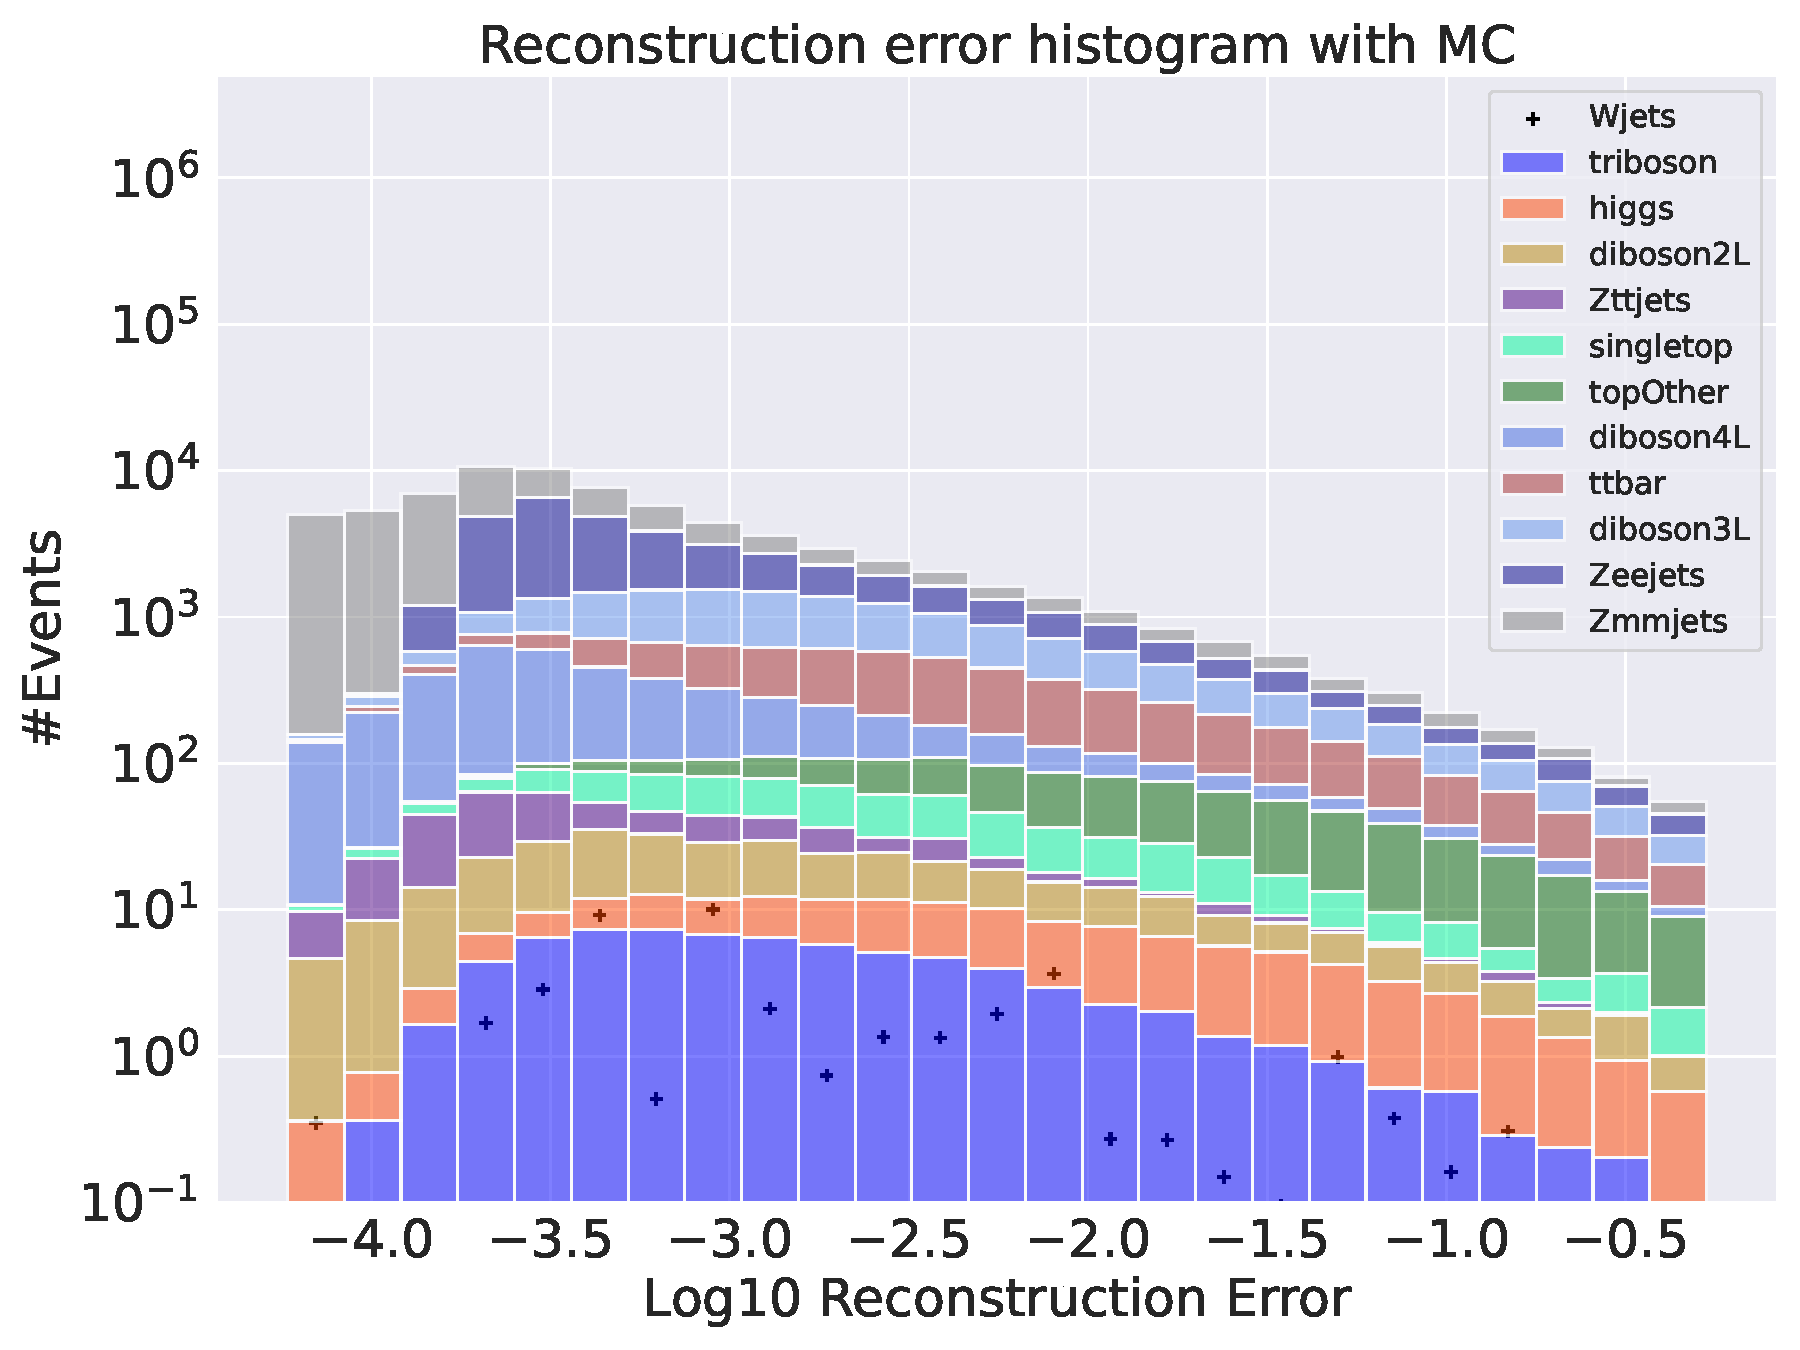
\includegraphics[width=\textwidth]{Figures/AE_testing/small/b_data_recon_big_rm3_feats_sig_Wjets.pdf}
        \caption{Reconstruction error on validation SM MC from the small Autoencoder. Here the Wjets channel has been removed from training and 
        is used as signal. No significant difference in distributions are found.}
        \label{fig:ae_small_Wjets}
    \end{subfigure}
    \hfill 
    \begin{subfigure}{.45\textwidth}
        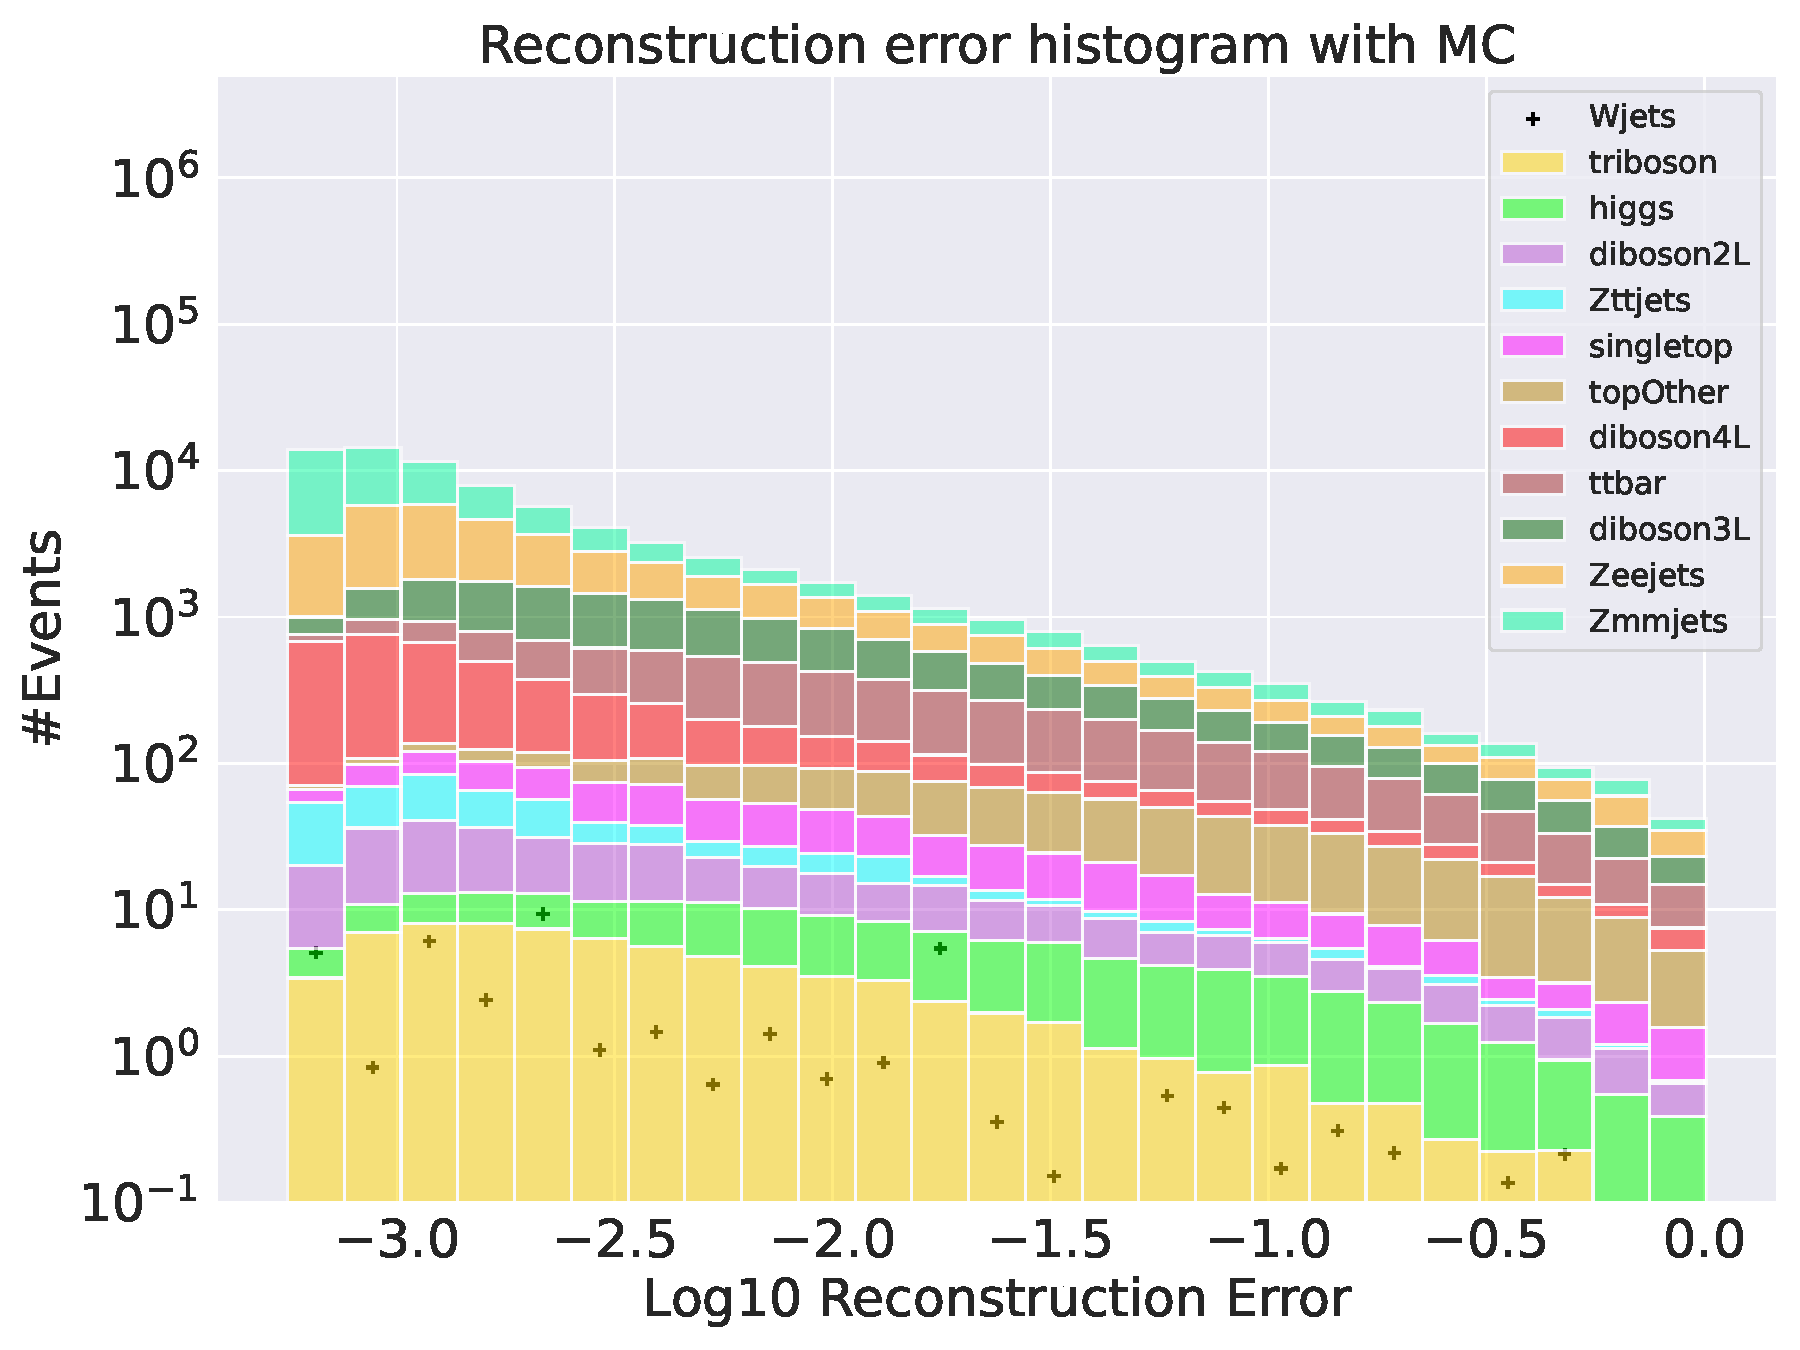
\includegraphics[width=\textwidth]{Figures/AE_testing/big/b_data_recon_big_rm3_feats_sig_Wjets.pdf}
        \caption{Reconstruction error on validation SM MC from the big Autoencoder. Here the Wjets channel has been removed from training and 
        is used as signal. No significant difference in distributions are found. }
        \label{fig:ae_big_Wjets}
    \end{subfigure}
    \hfill 
    \begin{subfigure}{.45\textwidth}
        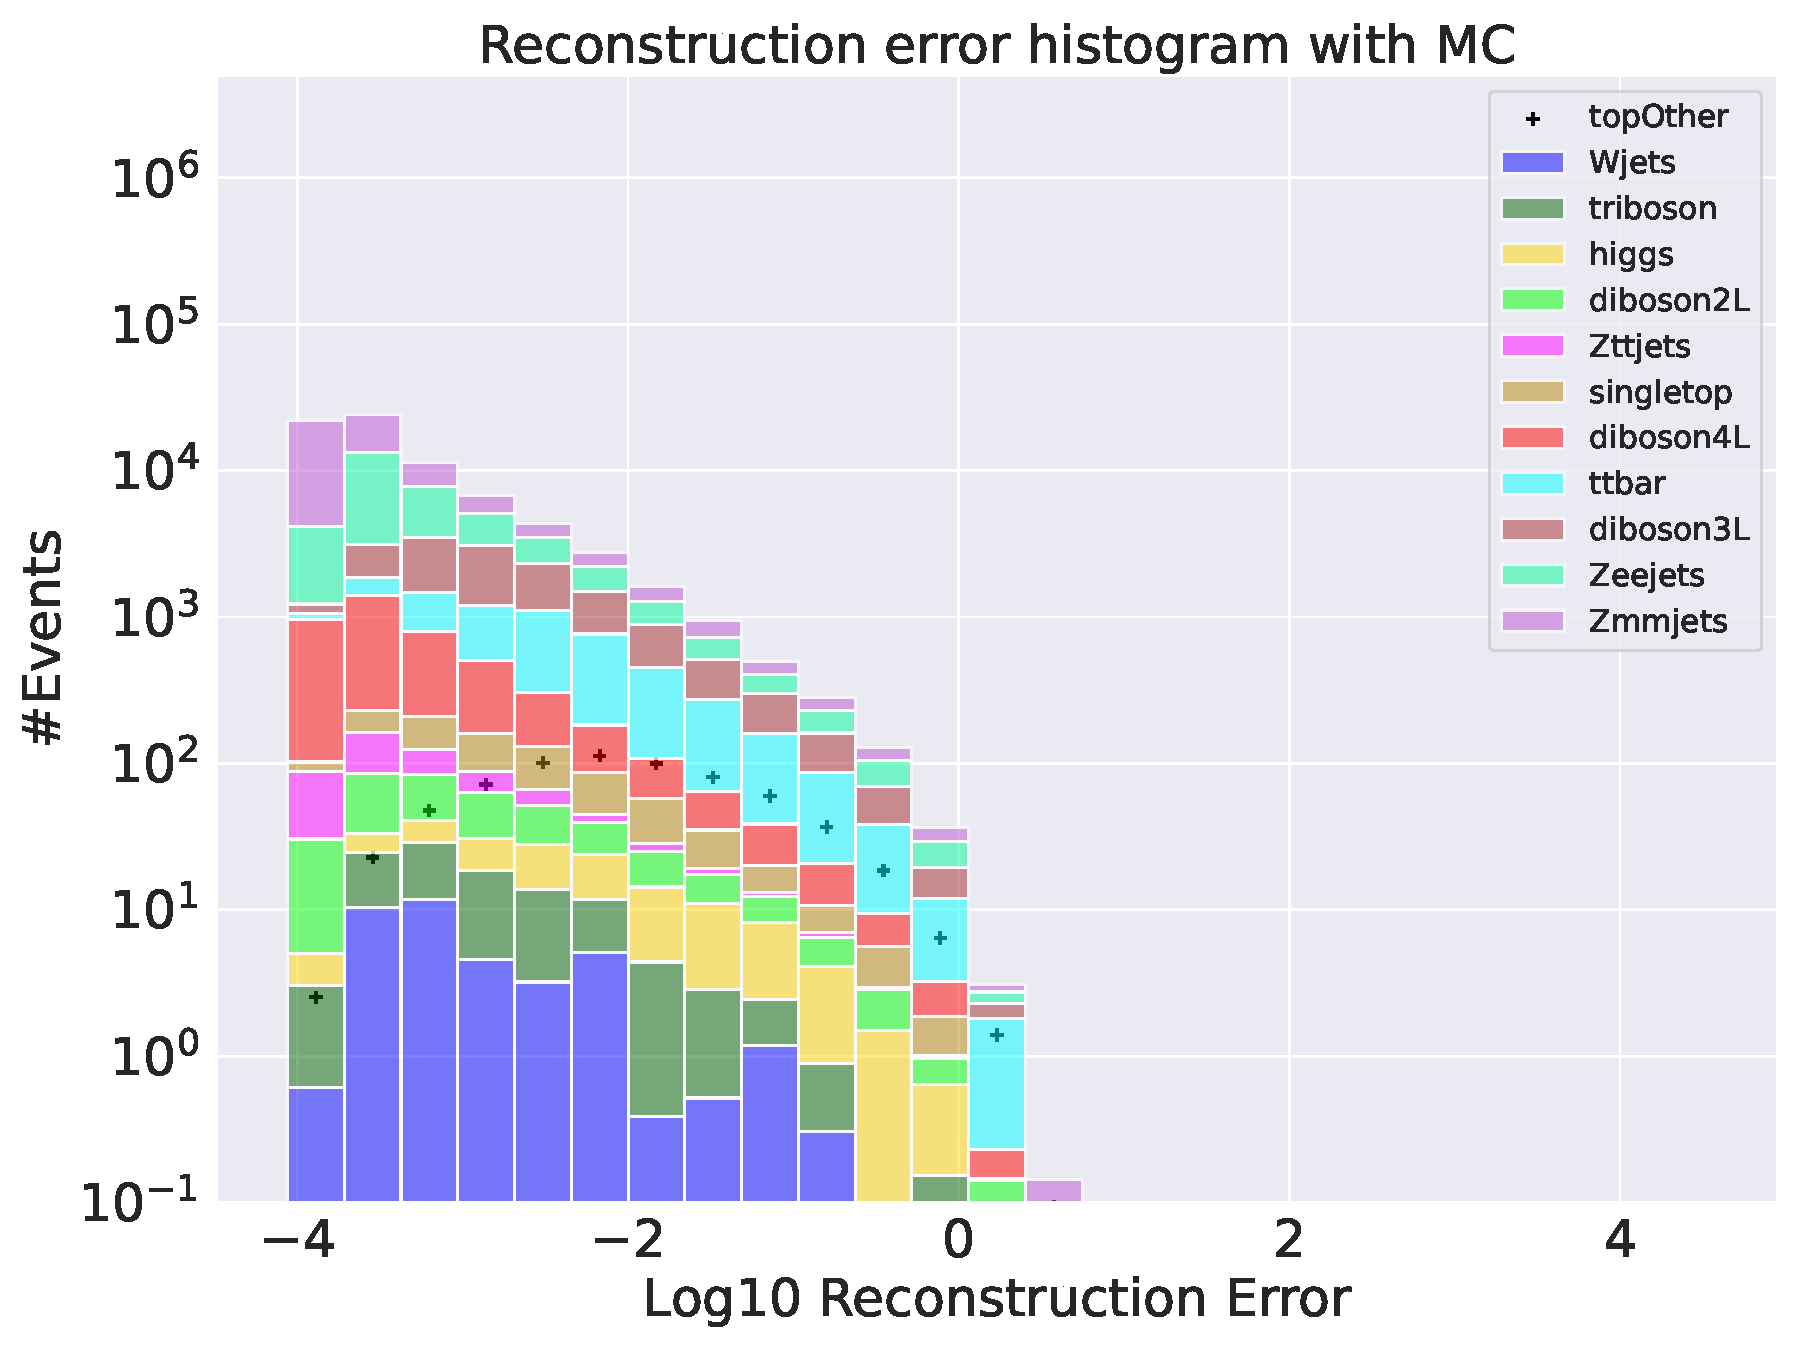
\includegraphics[width=\textwidth]{Figures/AE_testing/small/b_data_recon_big_rm3_feats_sig_topOther.pdf}
        \caption{Reconstruction error on validation SM MC from the small Autoencoder. Here the topOther channel has been removed from training and 
        is used as signal. No significant difference in distributions are found. }
        \label{fig:ae_small_topOther}
    \end{subfigure}
    \hfill
    \begin{subfigure}{.45\textwidth}
        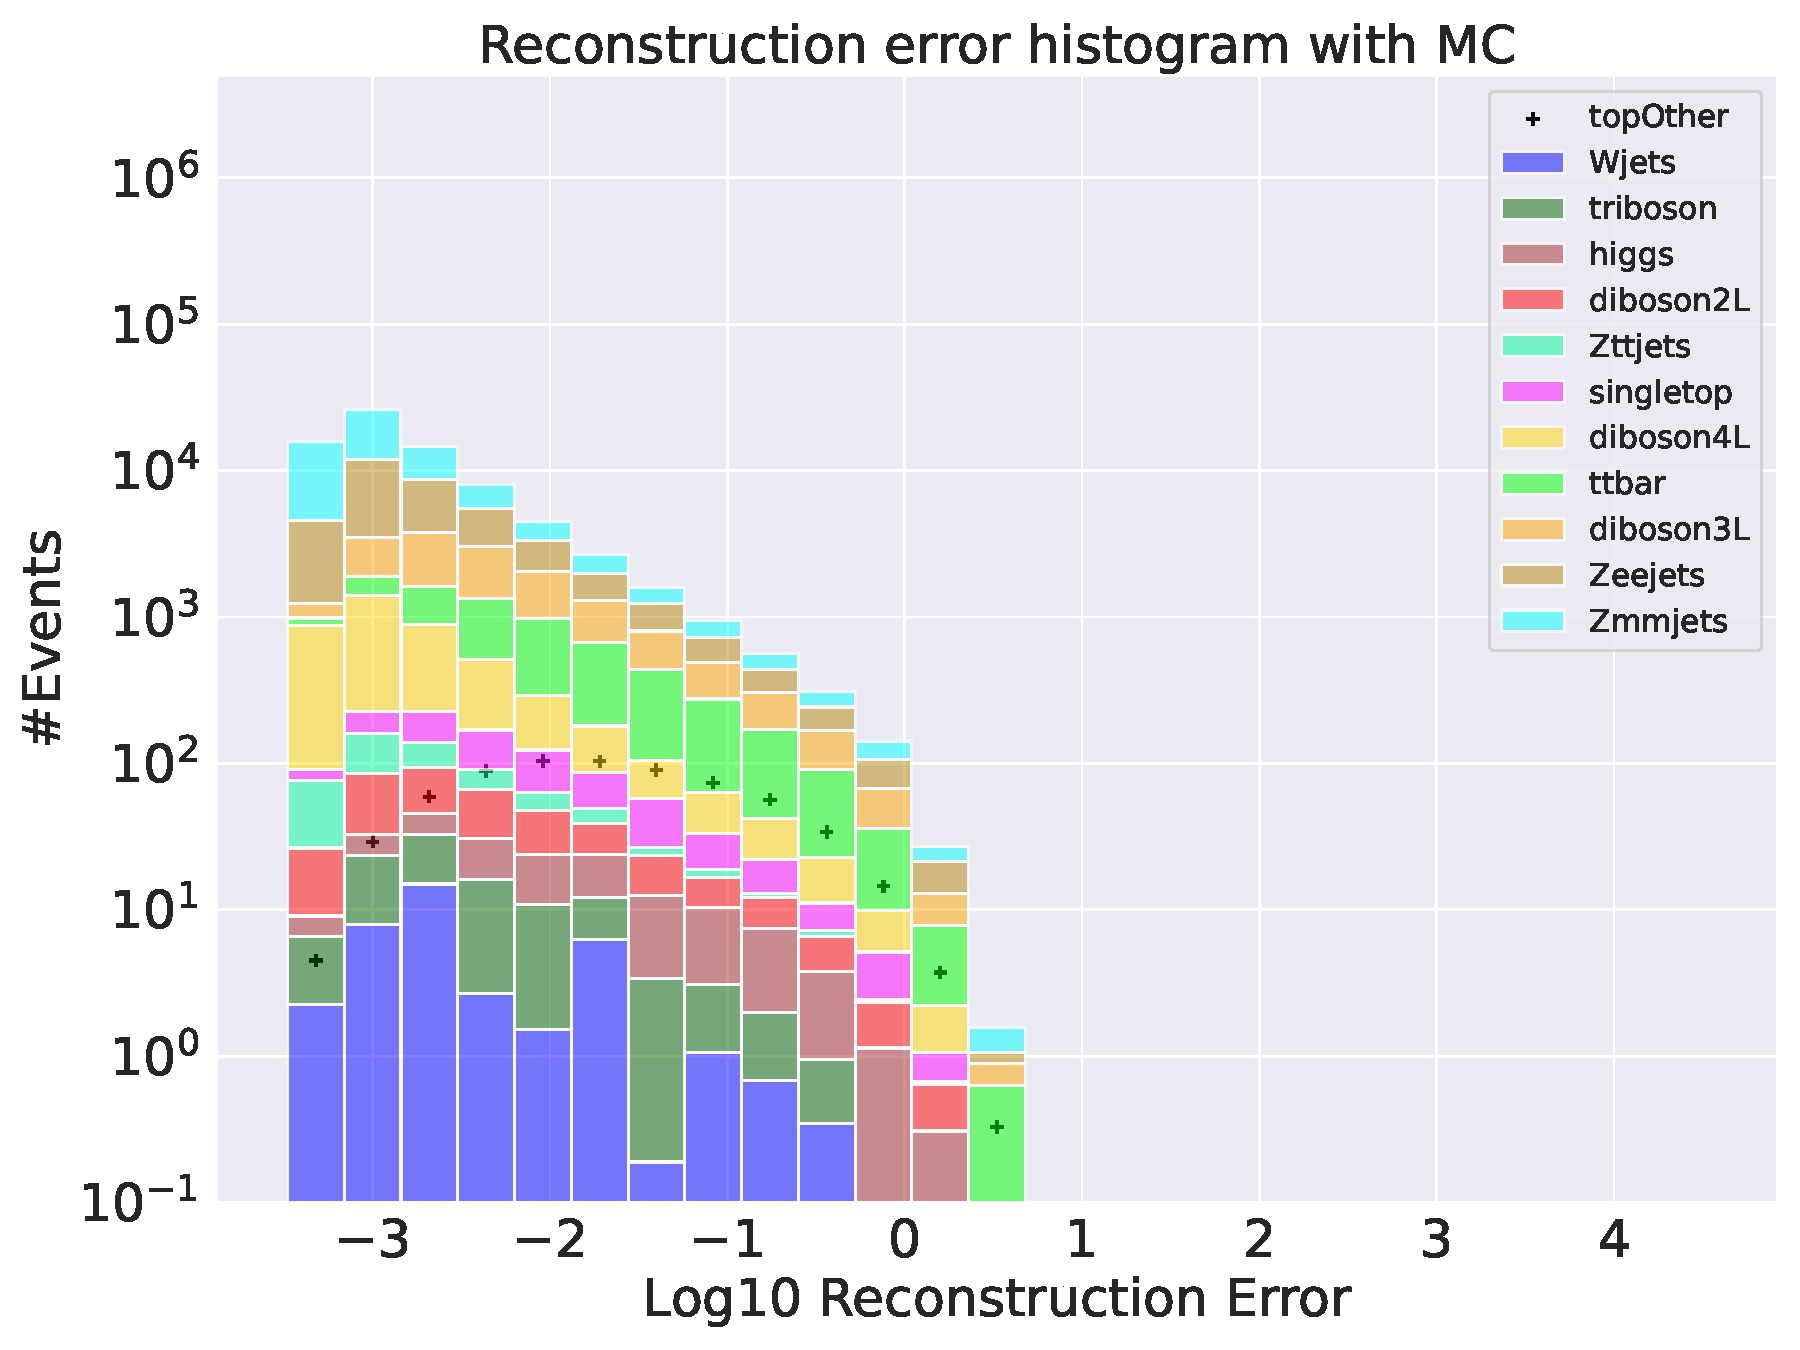
\includegraphics[width=\textwidth]{Figures/AE_testing/big/b_data_recon_big_rm3_feats_sig_topOther.pdf}
        \caption{Reconstruction error on validation SM MC from the big Autoencoder. Here the topOther channel has been removed from training and 
        is used as signal. No significant difference in distributions are found. }
        \label{fig:ae_big_topOther}
    \end{subfigure}
    \hfill
    \begin{subfigure}{.45\textwidth}
        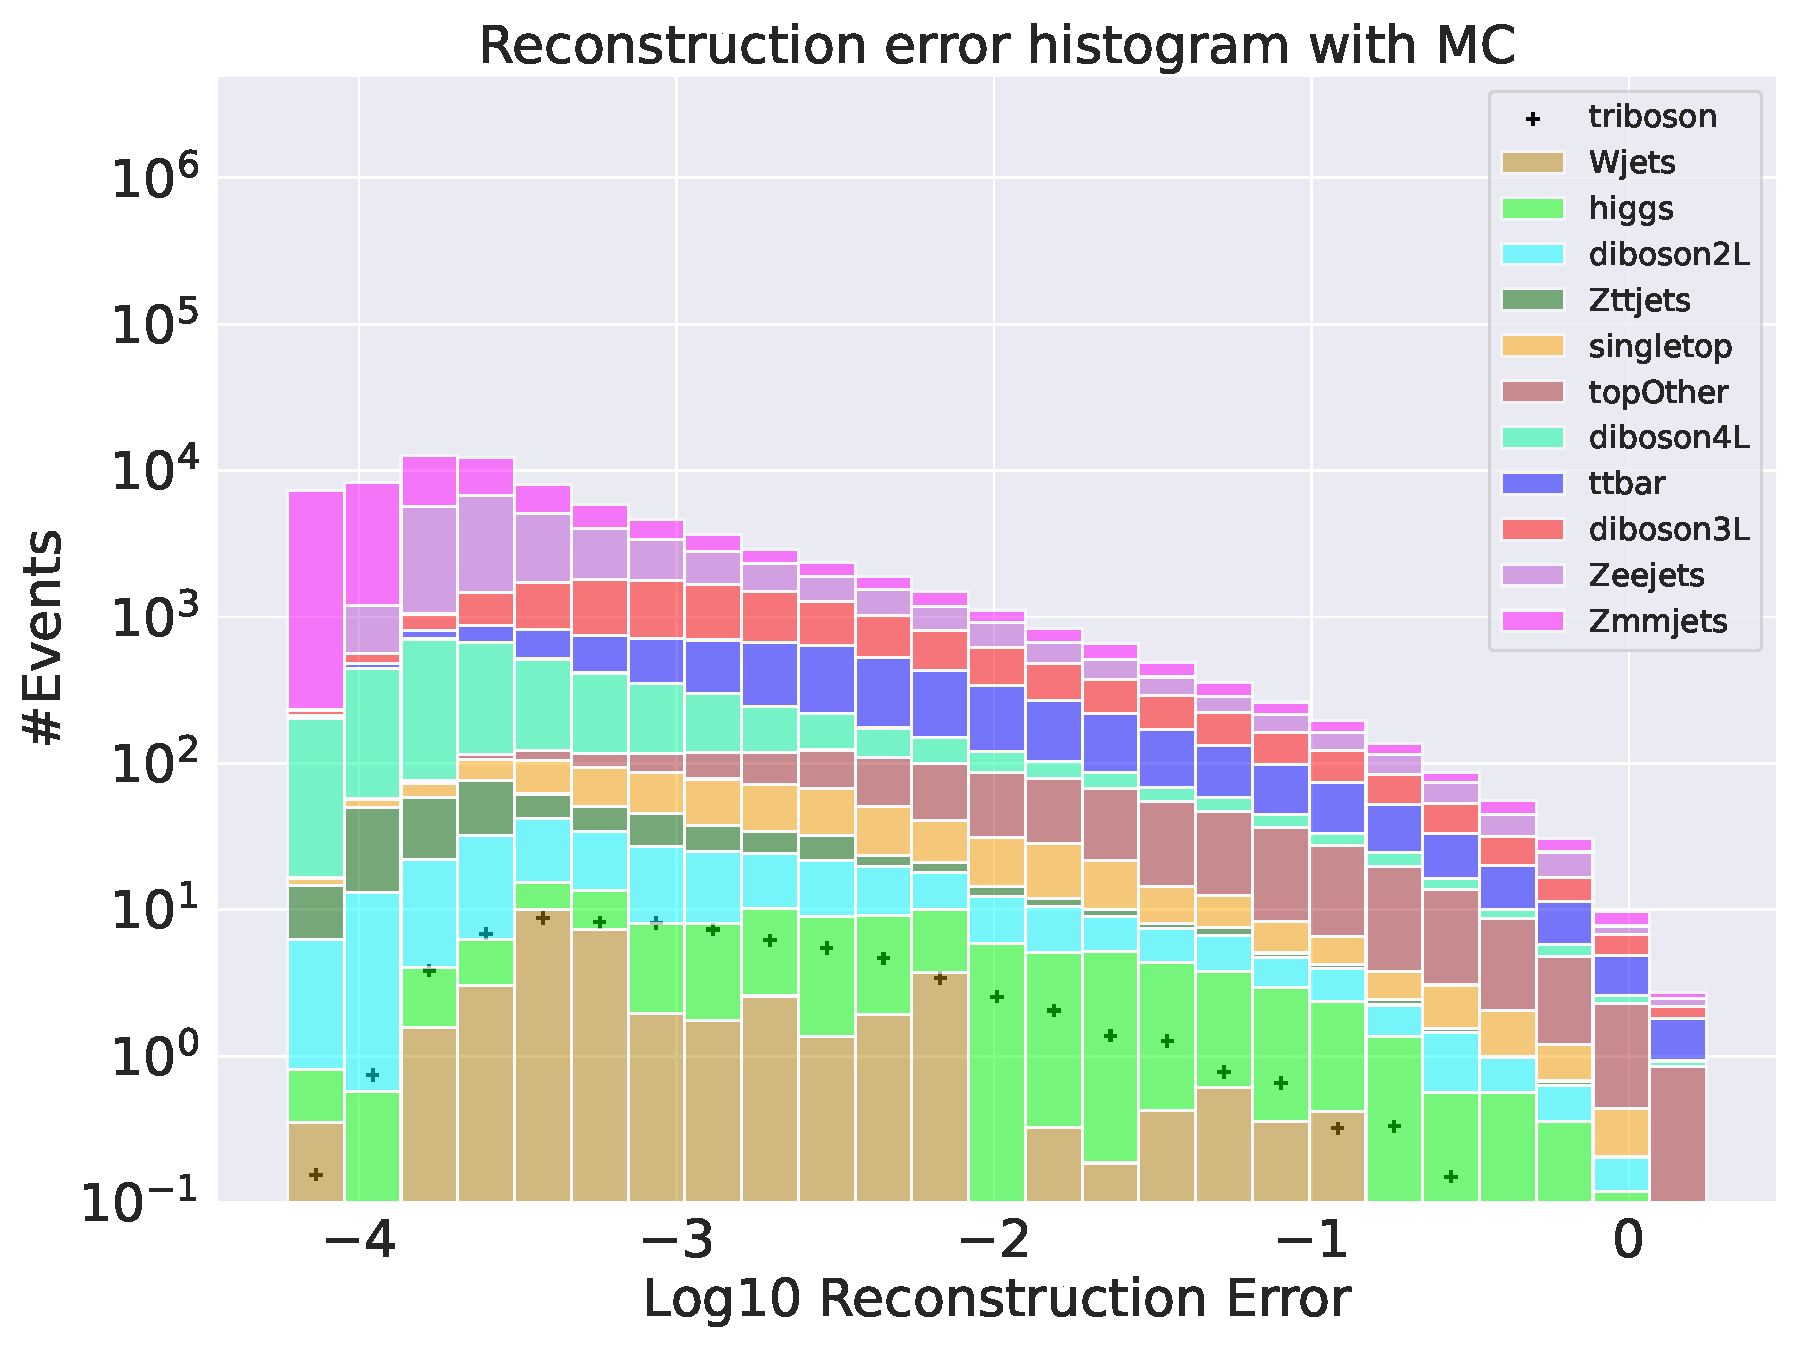
\includegraphics[width=\textwidth]{Figures/AE_testing/small/b_data_recon_big_rm3_feats_sig_triboson.pdf}
        \caption{Reconstruction error on validation SM MC from the small Autoencoder. Here the triboson channel has been removed from training and 
        is used as signal. No significant difference in distributions are found. }
        \label{fig:ae_small_triboson}
    \end{subfigure}
    \hfill 
    \begin{subfigure}{.45\textwidth}
        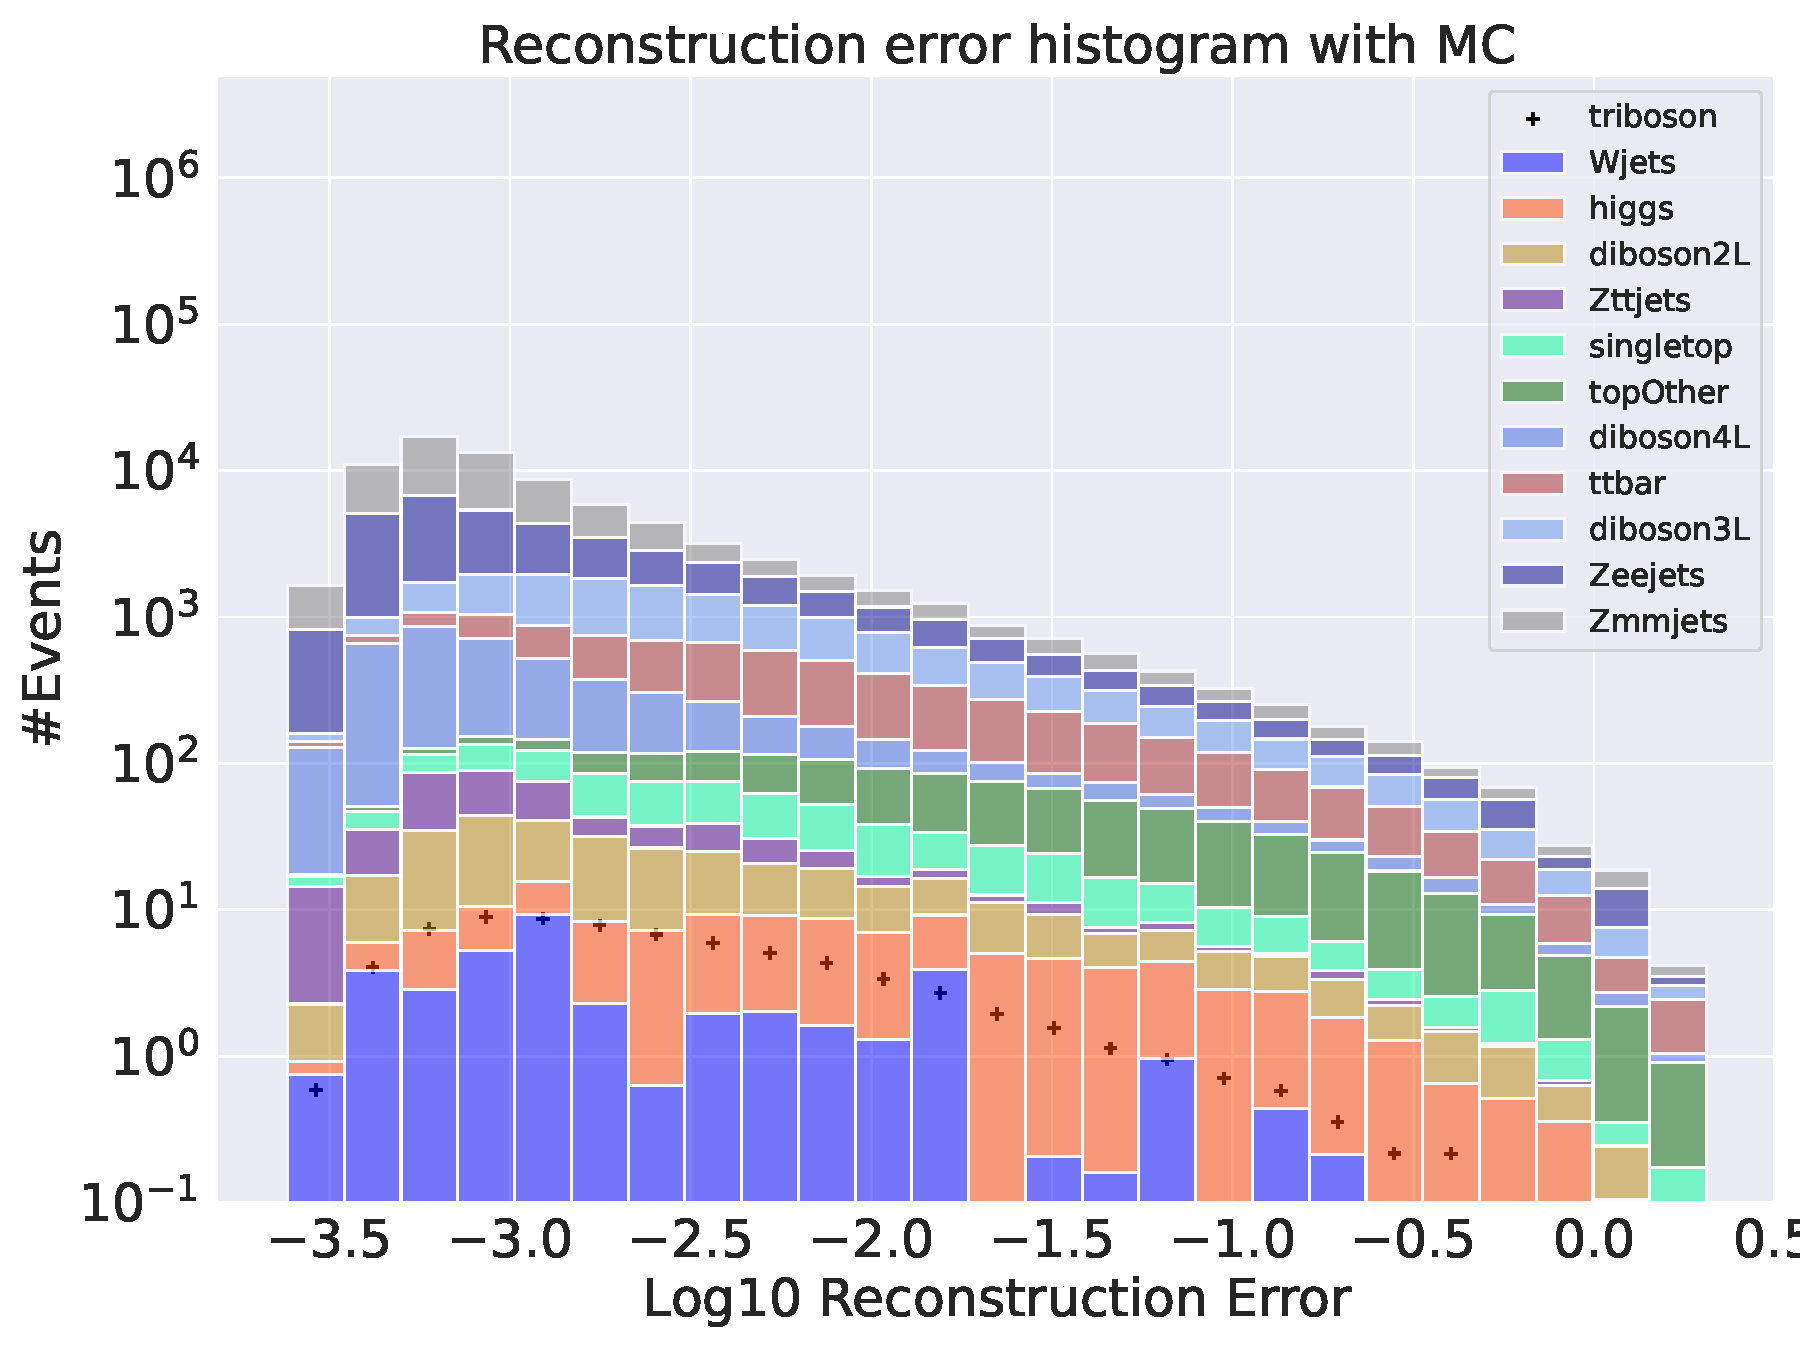
\includegraphics[width=\textwidth]{Figures/AE_testing/big/b_data_recon_big_rm3_feats_sig_triboson.pdf}
        \caption{Reconstruction error on validation SM MC from the big Autoencoder. Here the triboson channel has been removed from training and 
        is used as signal. No significant difference in distributions are found. }
        \label{fig:ae_big_triboson}
    \end{subfigure}
    \hfill  
    \caption{ }
    \label{fig:ae_big_channel4}
\end{figure}

\begin{figure}[H]
    \centering
    \begin{subfigure}{.45\textwidth}
        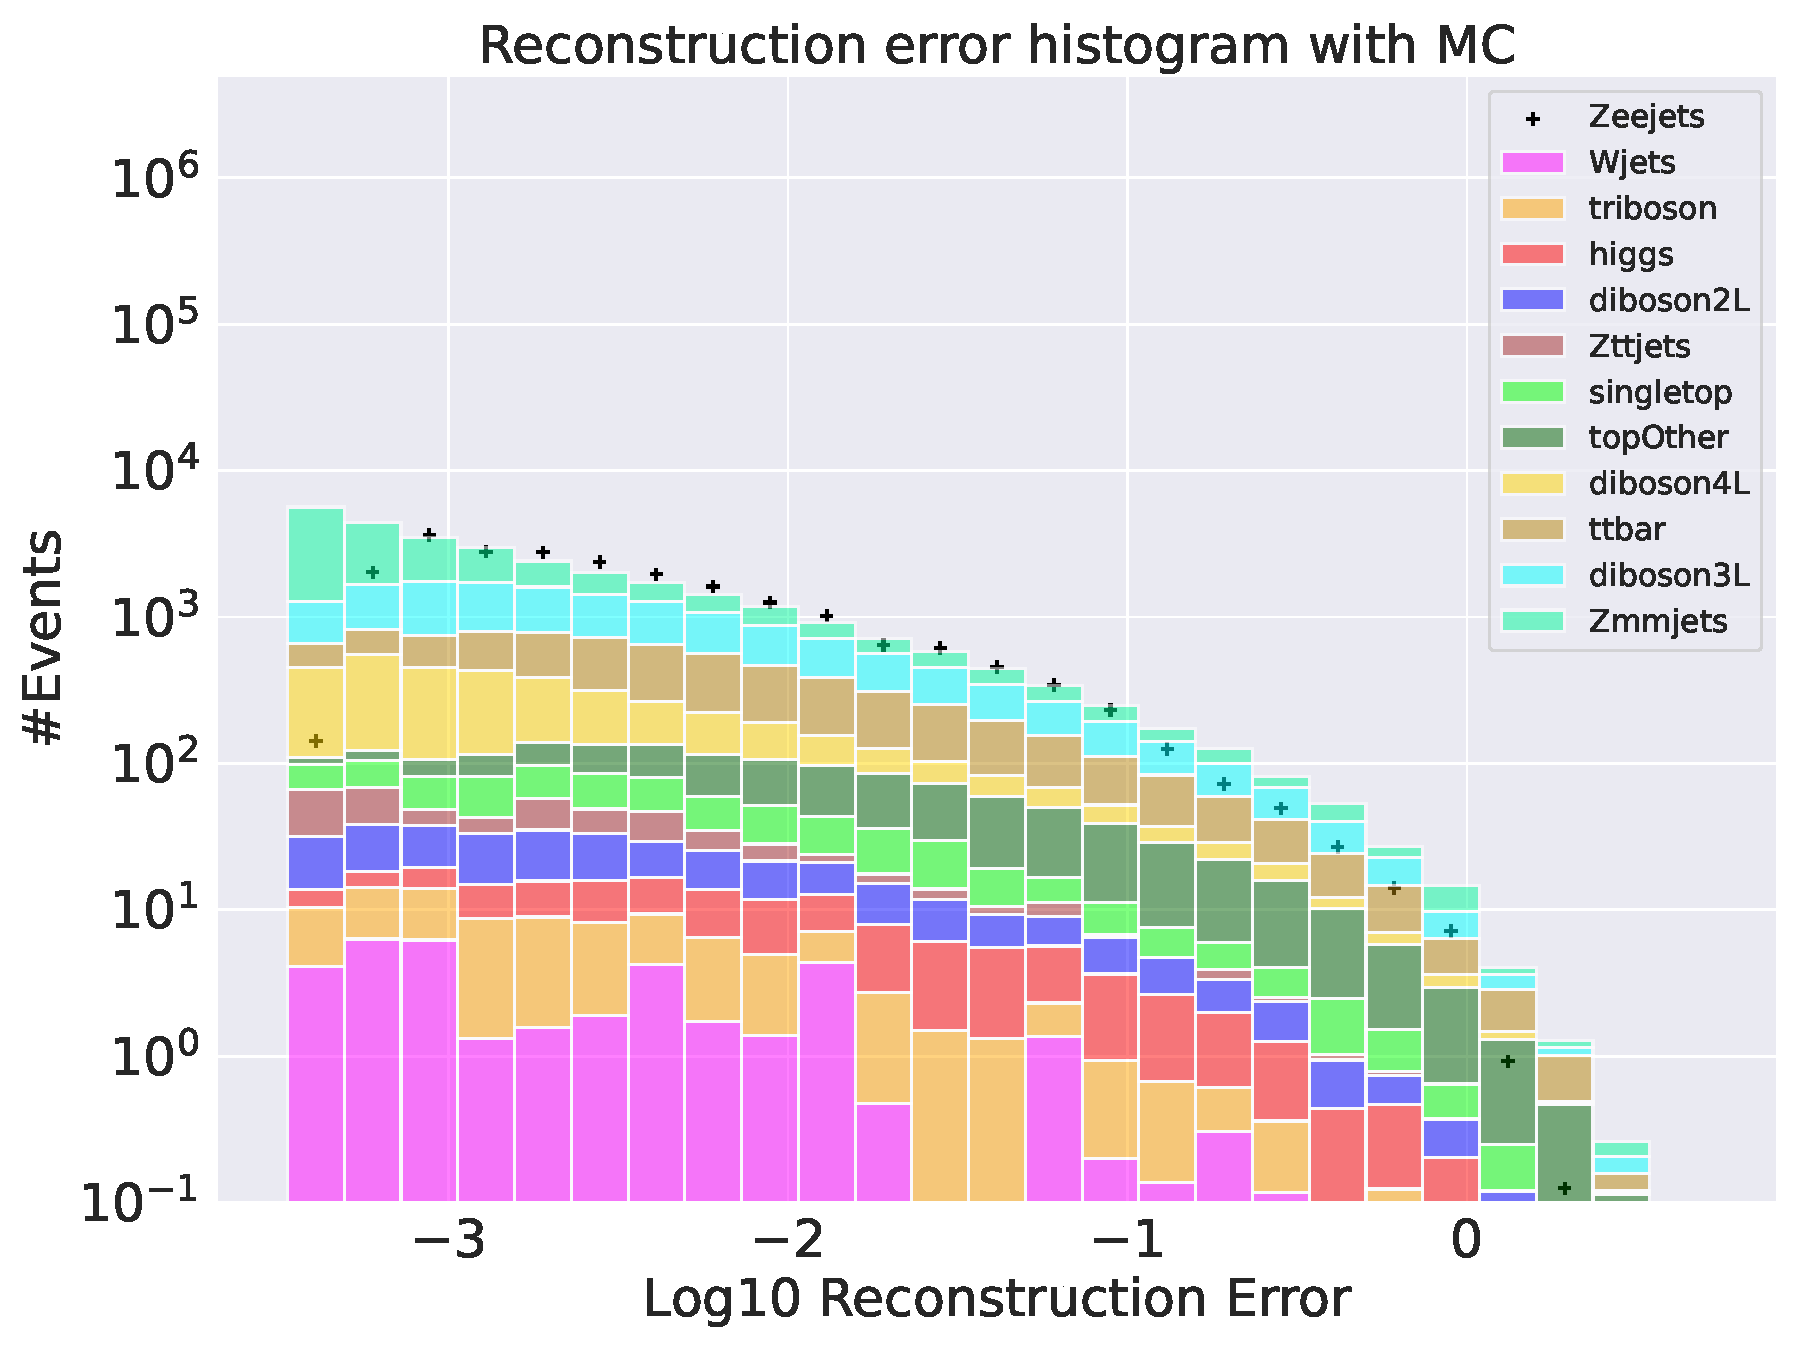
\includegraphics[width=\textwidth]{Figures/AE_testing/small/b_data_recon_big_rm3_feats_sig_Zeejets.pdf}
        \caption{Reconstruction error on validation SM MC from the small Autoencoder. Here the Zeejets channel has been removed from training and 
        is used as signal. No significant difference in distributions are found.}
        \label{fig:ae_small_Zeejets}
    \end{subfigure}
    \hfill 
    \begin{subfigure}{.45\textwidth}
        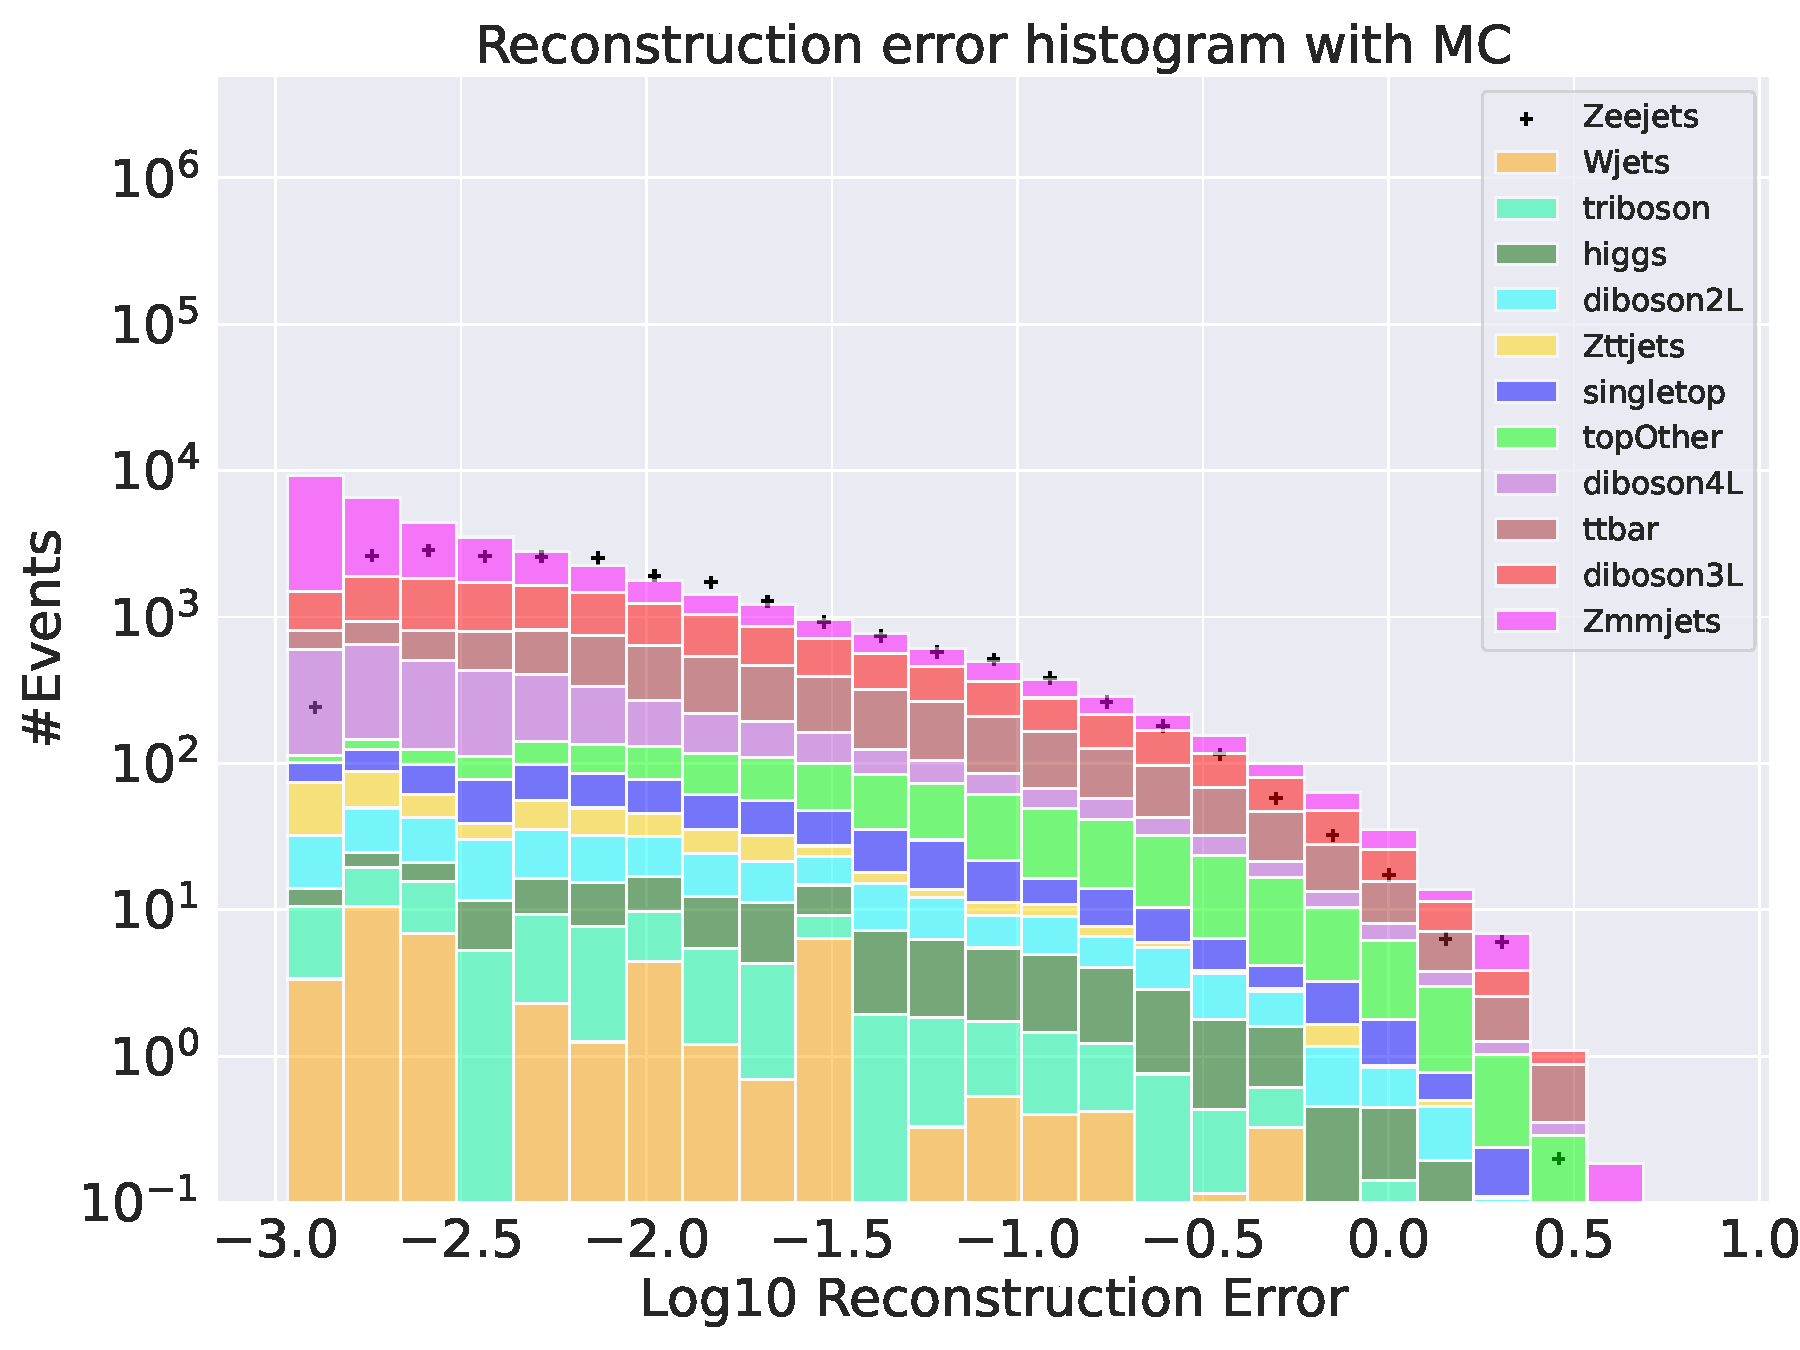
\includegraphics[width=\textwidth]{Figures/AE_testing/big/b_data_recon_big_rm3_feats_sig_Zeejets.pdf}
        \caption{Reconstruction error on validation SM MC from the big Autoencoder. Here the Zeejets channel has been removed from training and 
        is used as signal. No significant difference in distributions are found. }
        \label{fig:ae_big_Zeejets}
    \end{subfigure}
    \hfill 
    \begin{subfigure}{.45\textwidth}
        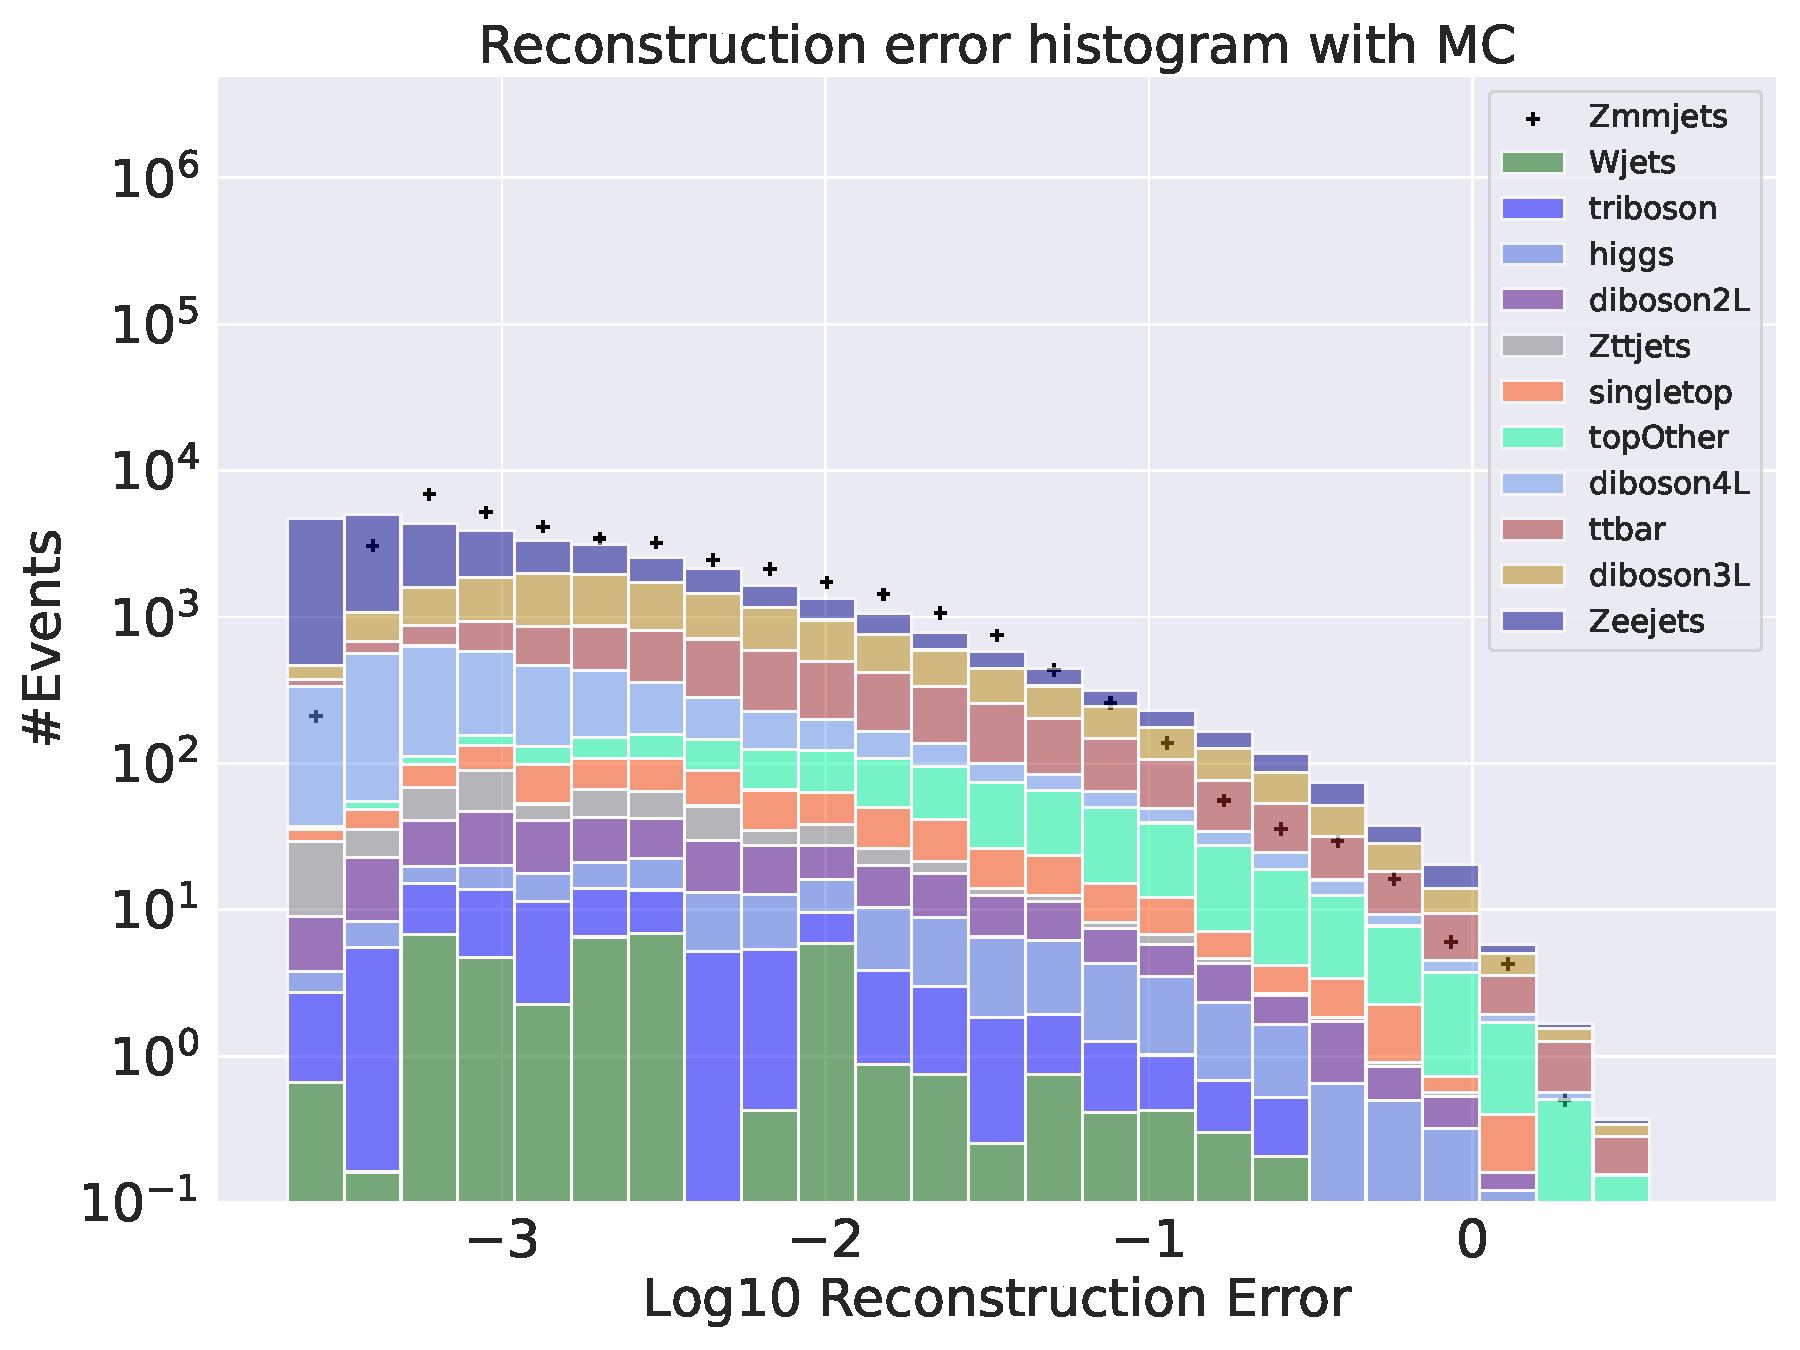
\includegraphics[width=\textwidth]{Figures/AE_testing/small/b_data_recon_big_rm3_feats_sig_Zmmjets.pdf}
        \caption{Reconstruction error on validation SM MC from the small Autoencoder. Here the Zmmjets channel has been removed from training and 
        is used as signal. No significant difference in distributions are found. }
        \label{fig:ae_small_Zmmjets}
    \end{subfigure}
    \hfill
    \begin{subfigure}{.45\textwidth}
        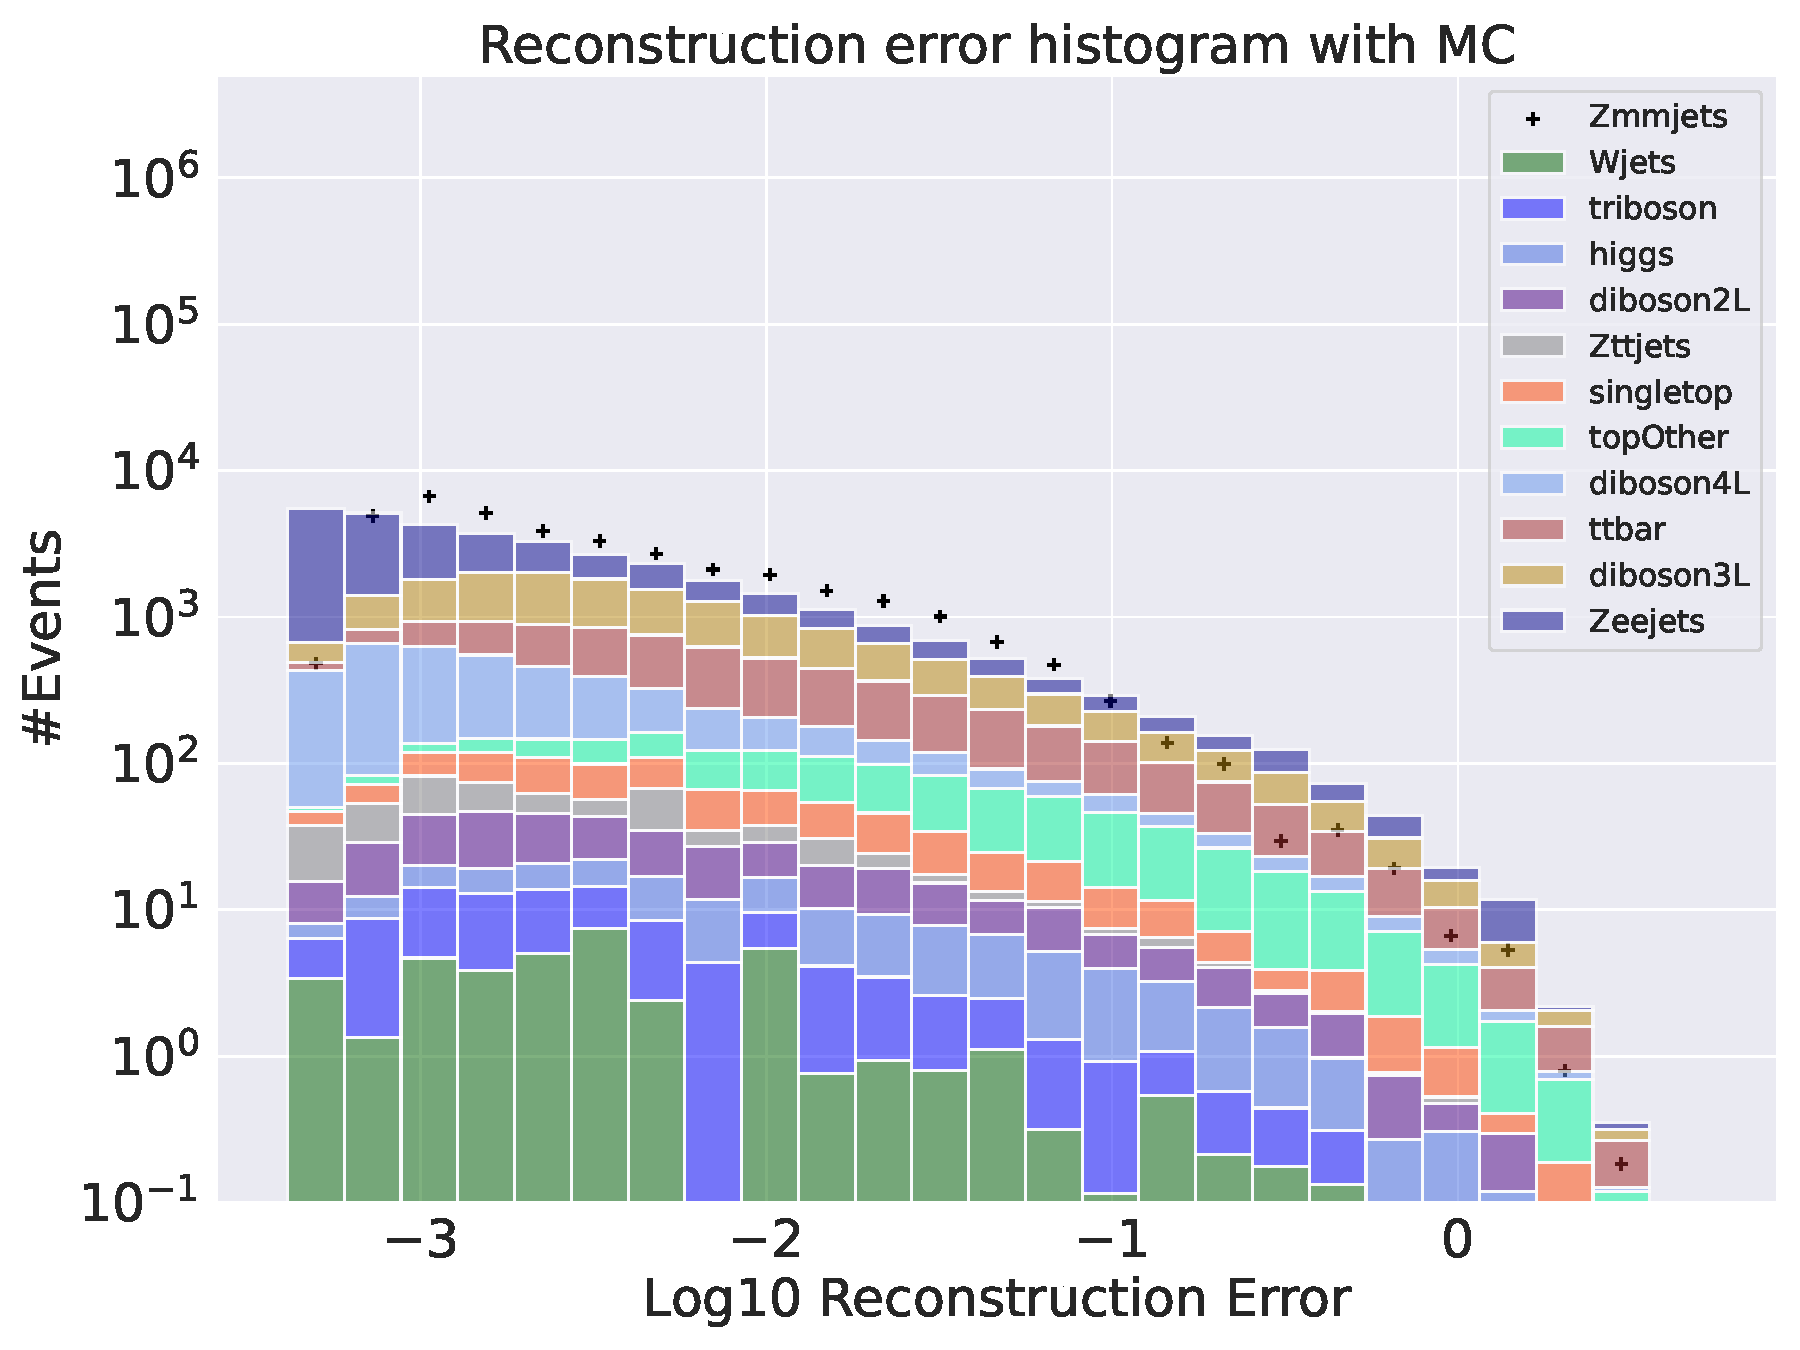
\includegraphics[width=\textwidth]{Figures/AE_testing/big/b_data_recon_big_rm3_feats_sig_Zmmjets.pdf}
        \caption{Reconstruction error on validation SM MC from the big Autoencoder. Here the Zmmjets channel has been removed from training and 
        is used as signal. No significant difference in distributions are found. }
        \label{fig:ae_big_Zmmjets}
    \end{subfigure}
    \hfill
    \begin{subfigure}{.45\textwidth}
        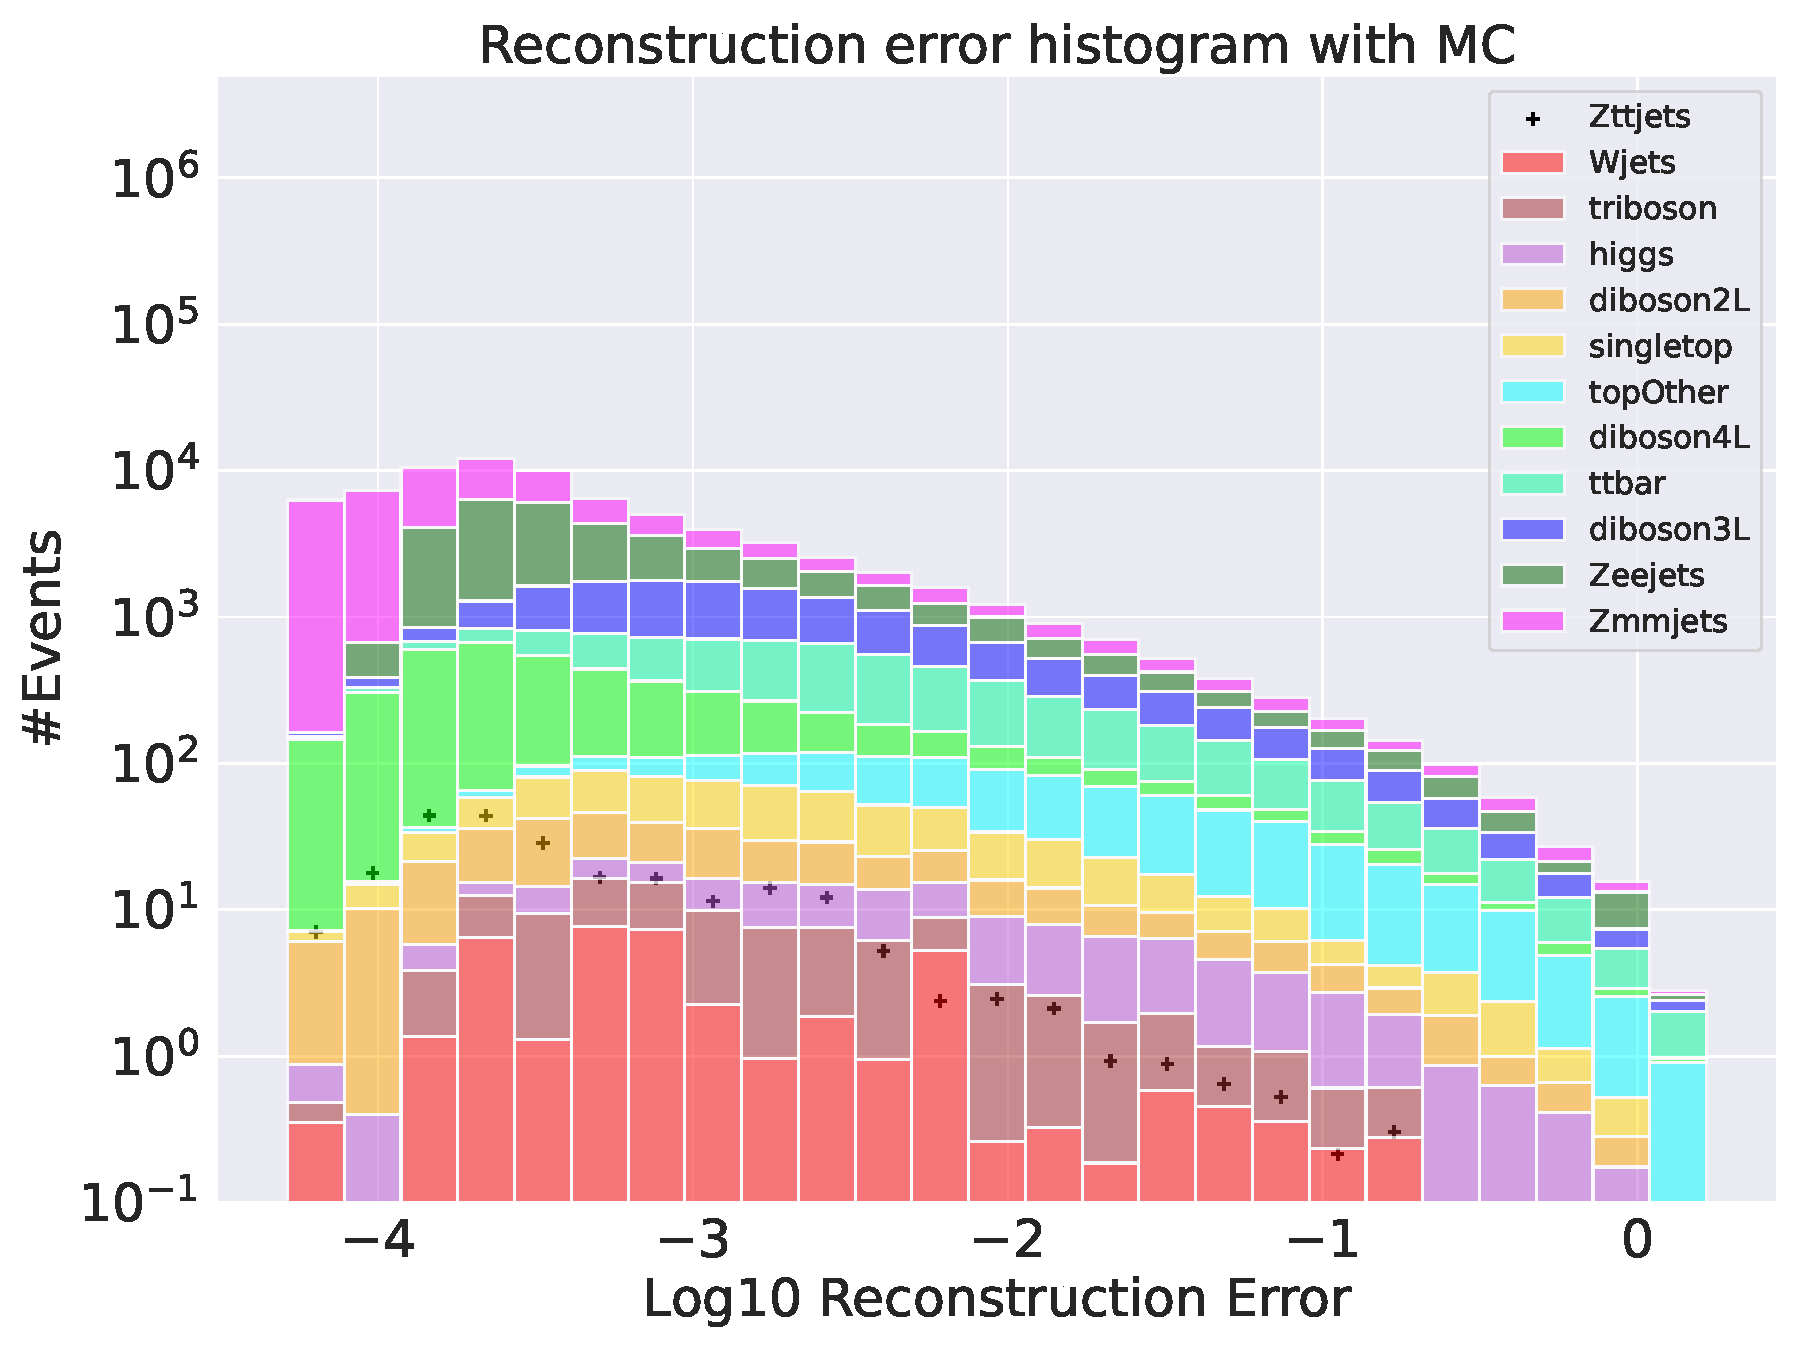
\includegraphics[width=\textwidth]{Figures/AE_testing/small/b_data_recon_big_rm3_feats_sig_Zttjets.pdf}
        \caption{Reconstruction error on validation SM MC from the small Autoencoder. Here the Zttjets channel has been removed from training and 
        is used as signal. No significant difference in distributions are found. }
        \label{fig:ae_small_Zttjets}
    \end{subfigure}
    \hfill 
    \begin{subfigure}{.45\textwidth}
        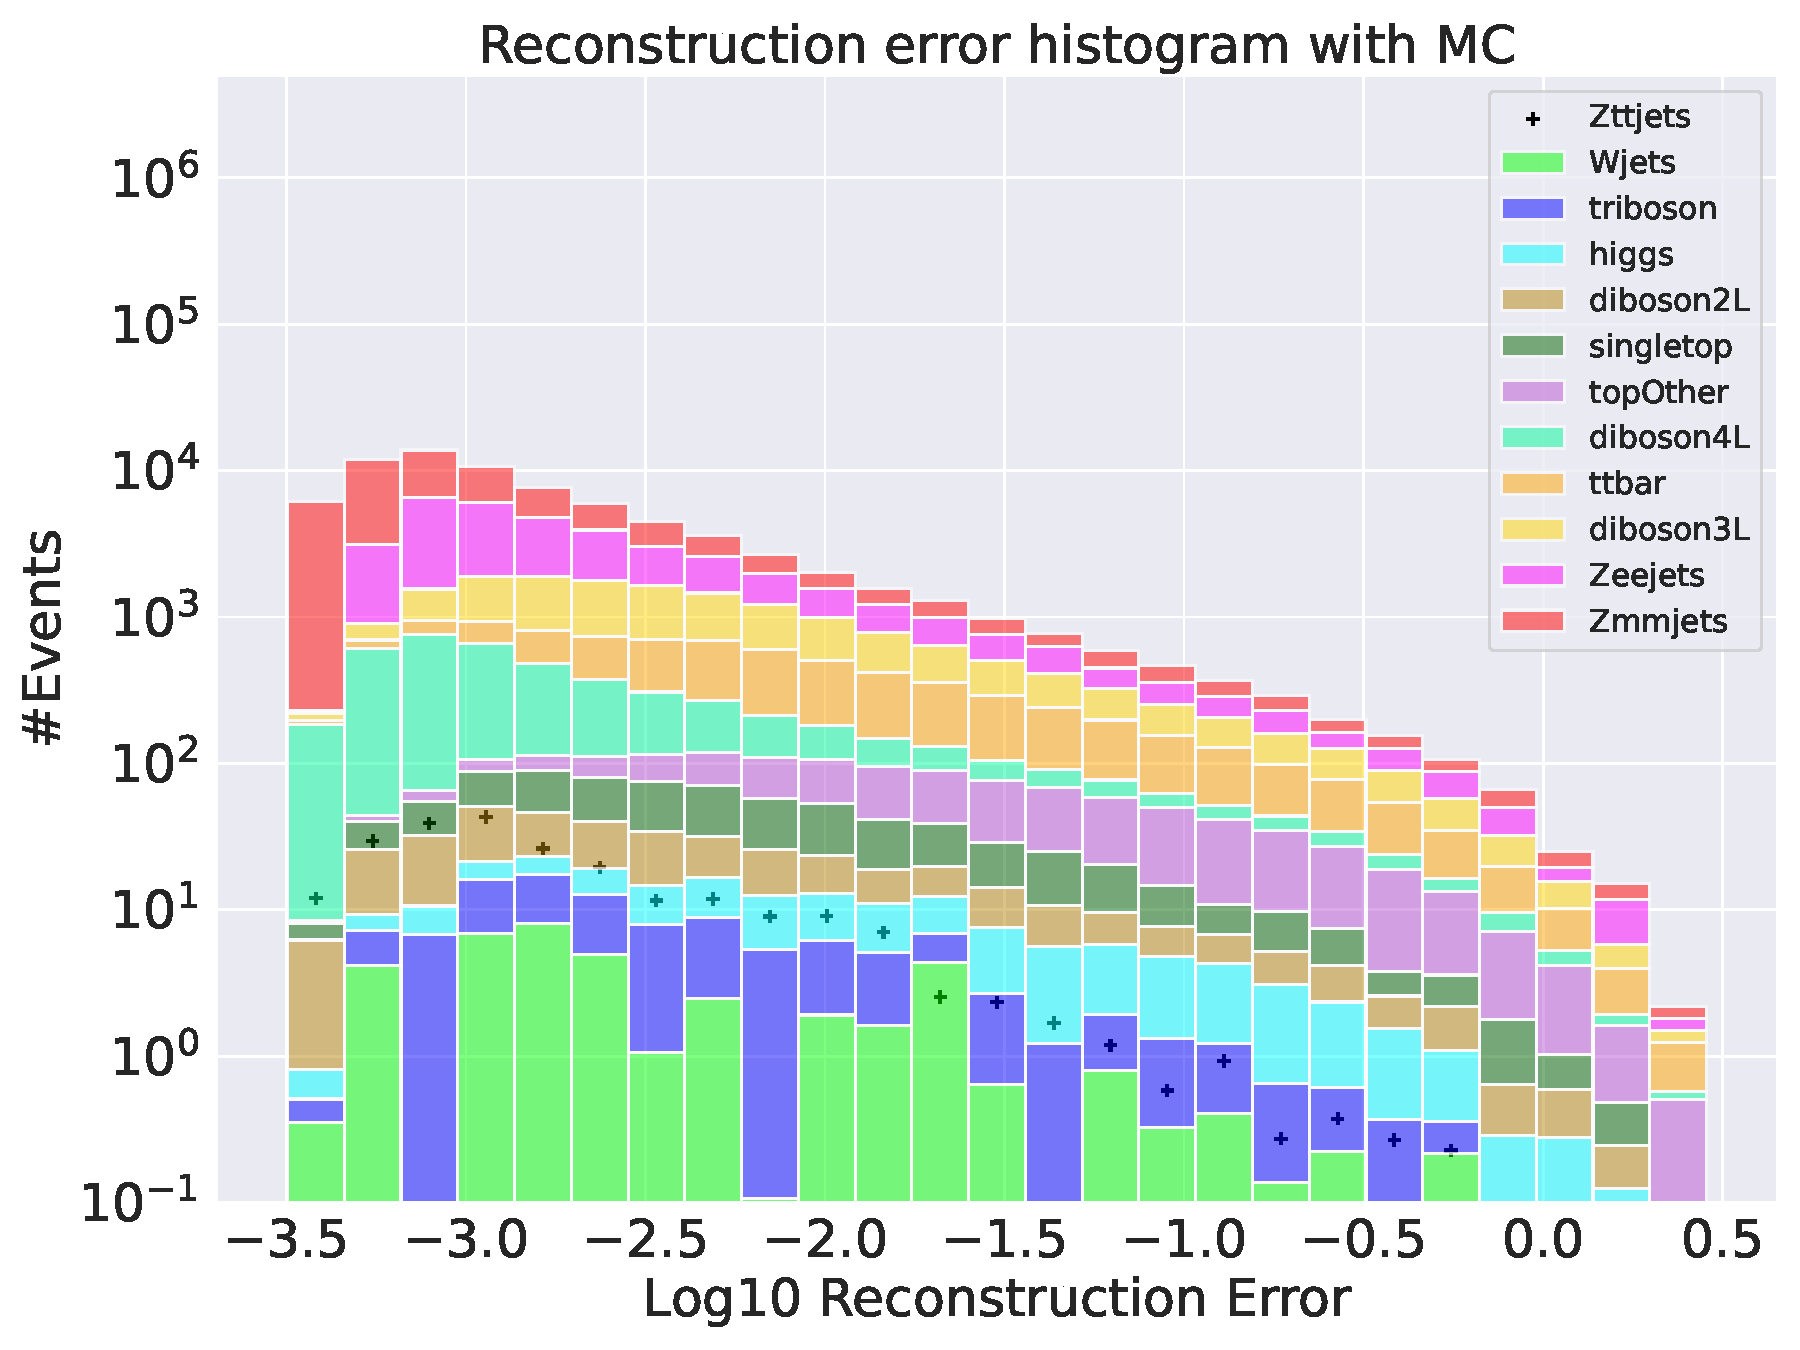
\includegraphics[width=\textwidth]{Figures/AE_testing/big/b_data_recon_big_rm3_feats_sig_Zttjets.pdf}
        \caption{Reconstruction error on validation SM MC from the big Autoencoder. Here the Zttjets channel has been removed from training and 
        is used as signal. No significant difference in distributions are found. }
        \label{fig:ae_big_Zttjets}
    \end{subfigure}
    \hfill  
    \caption{ }
    \label{fig:ae_big_channel5}
\end{figure}

\subsubsection*{Variational autoencoder}

\begin{figure}[H]
    \centering
    \begin{subfigure}{.45\textwidth}
        \includegraphics[width=\textwidth]{Figures/VAE_testing/small/b_data_recon_big_rm3_feats_sig_diboson2l.pdf}
        \caption{Reconstruction error on validation SM MC from the small Autoencoder. Here the diboson2l channel has been removed from training and 
        is used as signal. No significant difference in distributions are found.}
        \label{fig:vae_small_diboson2l}
    \end{subfigure}
    \hfill 
    \begin{subfigure}{.45\textwidth}
        \includegraphics[width=\textwidth]{Figures/VAE_testing/big/b_data_recon_big_rm3_feats_sig_diboson2l.pdf}
        \caption{Reconstruction error on validation SM MC from the big Autoencoder. Here the diboson2l channel has been removed from training and 
        is used as signal. No significant difference in distributions are found. }
        \label{fig:vae_big_diboson2l}
    \end{subfigure}
    \hfill 
    \begin{subfigure}{.45\textwidth}
        \includegraphics[width=\textwidth]{Figures/VAE_testing/small/b_data_recon_big_rm3_feats_sig_diboson3l.pdf}
        \caption{Reconstruction error on validation SM MC from the small Autoencoder. Here the diboson3l channel has been removed from training and 
        is used as signal. No significant difference in distributions are found. }
        \label{fig:vae_small_diboson3l}
    \end{subfigure}
    \hfill
    \begin{subfigure}{.45\textwidth}
        \includegraphics[width=\textwidth]{Figures/VAE_testing/big/b_data_recon_big_rm3_feats_sig_diboson3l.pdf}
        \caption{Reconstruction error on validation SM MC from the big Autoencoder. Here the diboson3l channel has been removed from training and 
        is used as signal. No significant difference in distributions are found. }
        \label{fig:vae_big_diboson3l}
    \end{subfigure}
    \hfill
    \begin{subfigure}{.45\textwidth}
        \includegraphics[width=\textwidth]{Figures/VAE_testing/small/b_data_recon_big_rm3_feats_sig_diboson4l.pdf}
        \caption{Reconstruction error on validation SM MC from the small Autoencoder. Here the diboson4l channel has been removed from training and 
        is used as signal. No significant difference in distributions are found. }
        \label{fig:vae_small_diboson4l}
    \end{subfigure}
    \hfill 
    \begin{subfigure}{.45\textwidth}
        \includegraphics[width=\textwidth]{Figures/VAE_testing/big/b_data_recon_big_rm3_feats_sig_diboson4l.pdf}
        \caption{Reconstruction error on validation SM MC from the big Autoencoder. Here the diboson4l channel has been removed from training and 
        is used as signal. No significant difference in distributions are found. }
        \label{fig:vae_big_diboson4l}
    \end{subfigure}
    \hfill  
    \caption{ }
    \label{fig:vae_big_channel3}
\end{figure}


\begin{figure}[H]
    \centering
    \begin{subfigure}{.45\textwidth}
        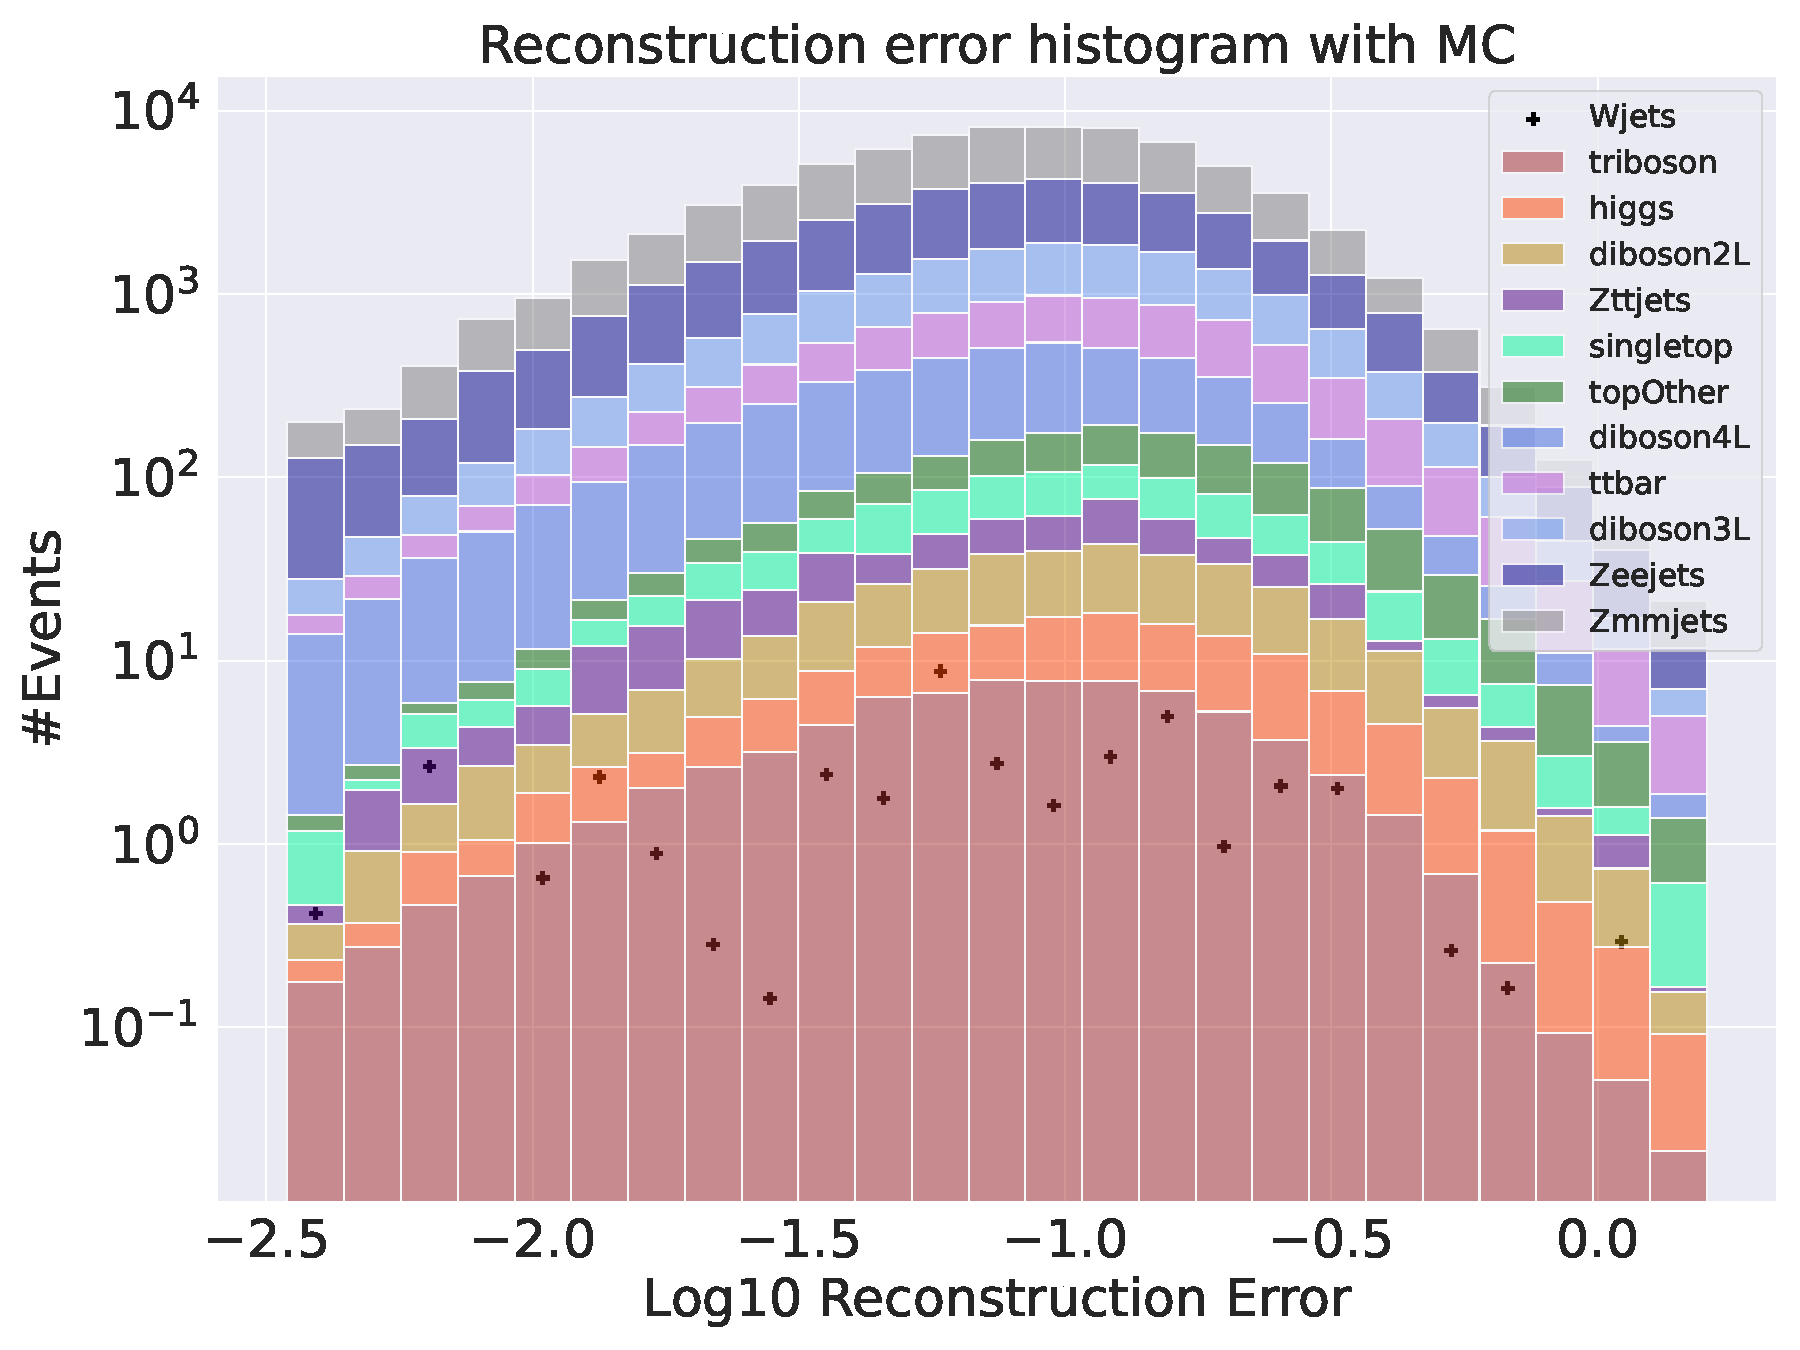
\includegraphics[width=\textwidth]{Figures/VAE_testing/small/b_data_recon_big_rm3_feats_sig_Wjets.pdf}
        \caption{Reconstruction error on validation SM MC from the small Autoencoder. Here the Wjets channel has been removed from training and 
        is used as signal. No significant difference in distributions are found.}
        \label{fig:vae_small_Wjets}
    \end{subfigure}
    \hfill 
    \begin{subfigure}{.45\textwidth}
        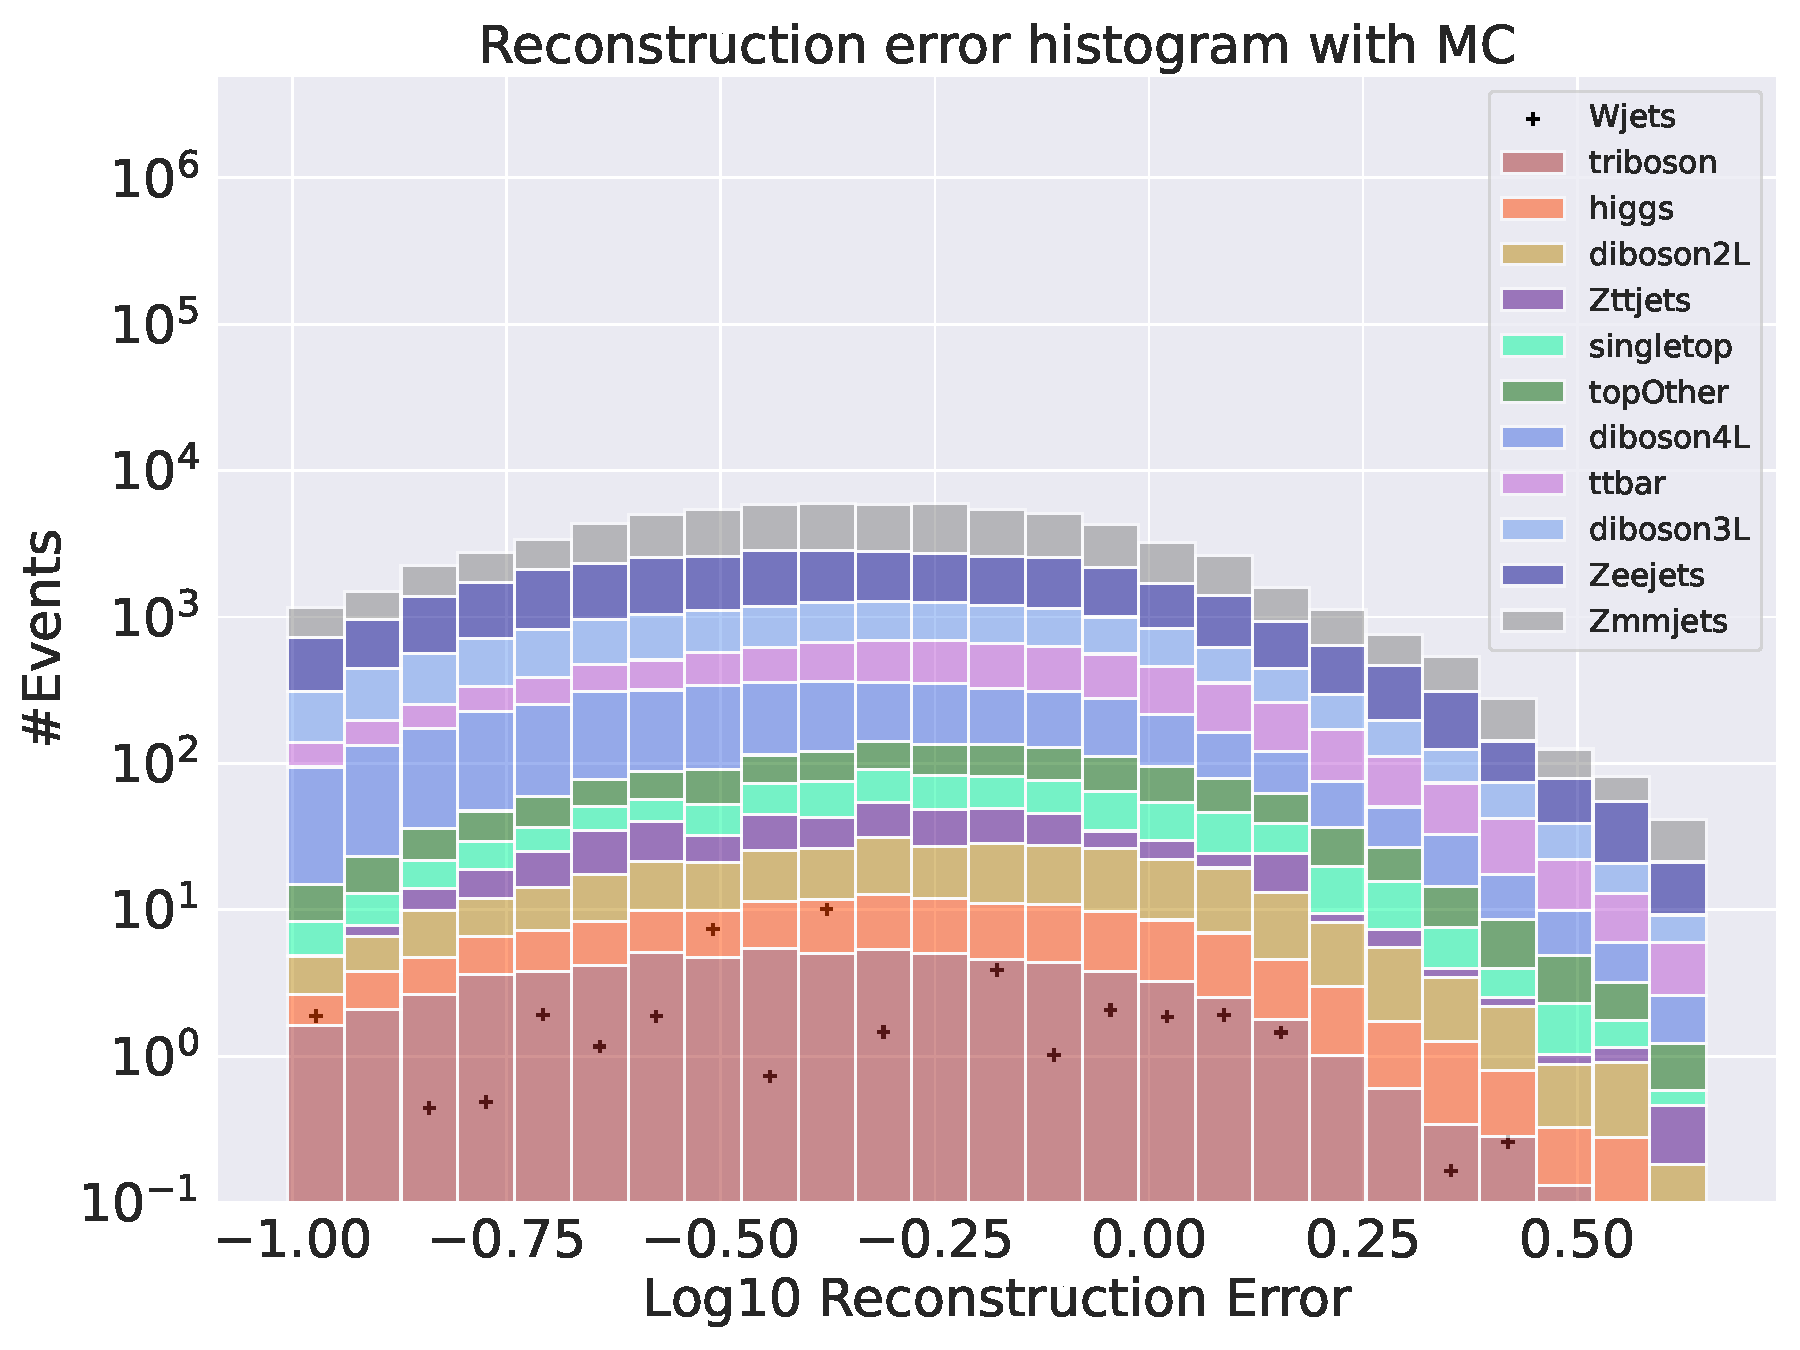
\includegraphics[width=\textwidth]{Figures/VAE_testing/big/b_data_recon_big_rm3_feats_sig_Wjets.pdf}
        \caption{Reconstruction error on validation SM MC from the big Autoencoder. Here the Wjets channel has been removed from training and 
        is used as signal. No significant difference in distributions are found. }
        \label{fig:vae_big_Wjets}
    \end{subfigure}
    \hfill 
    \begin{subfigure}{.45\textwidth}
        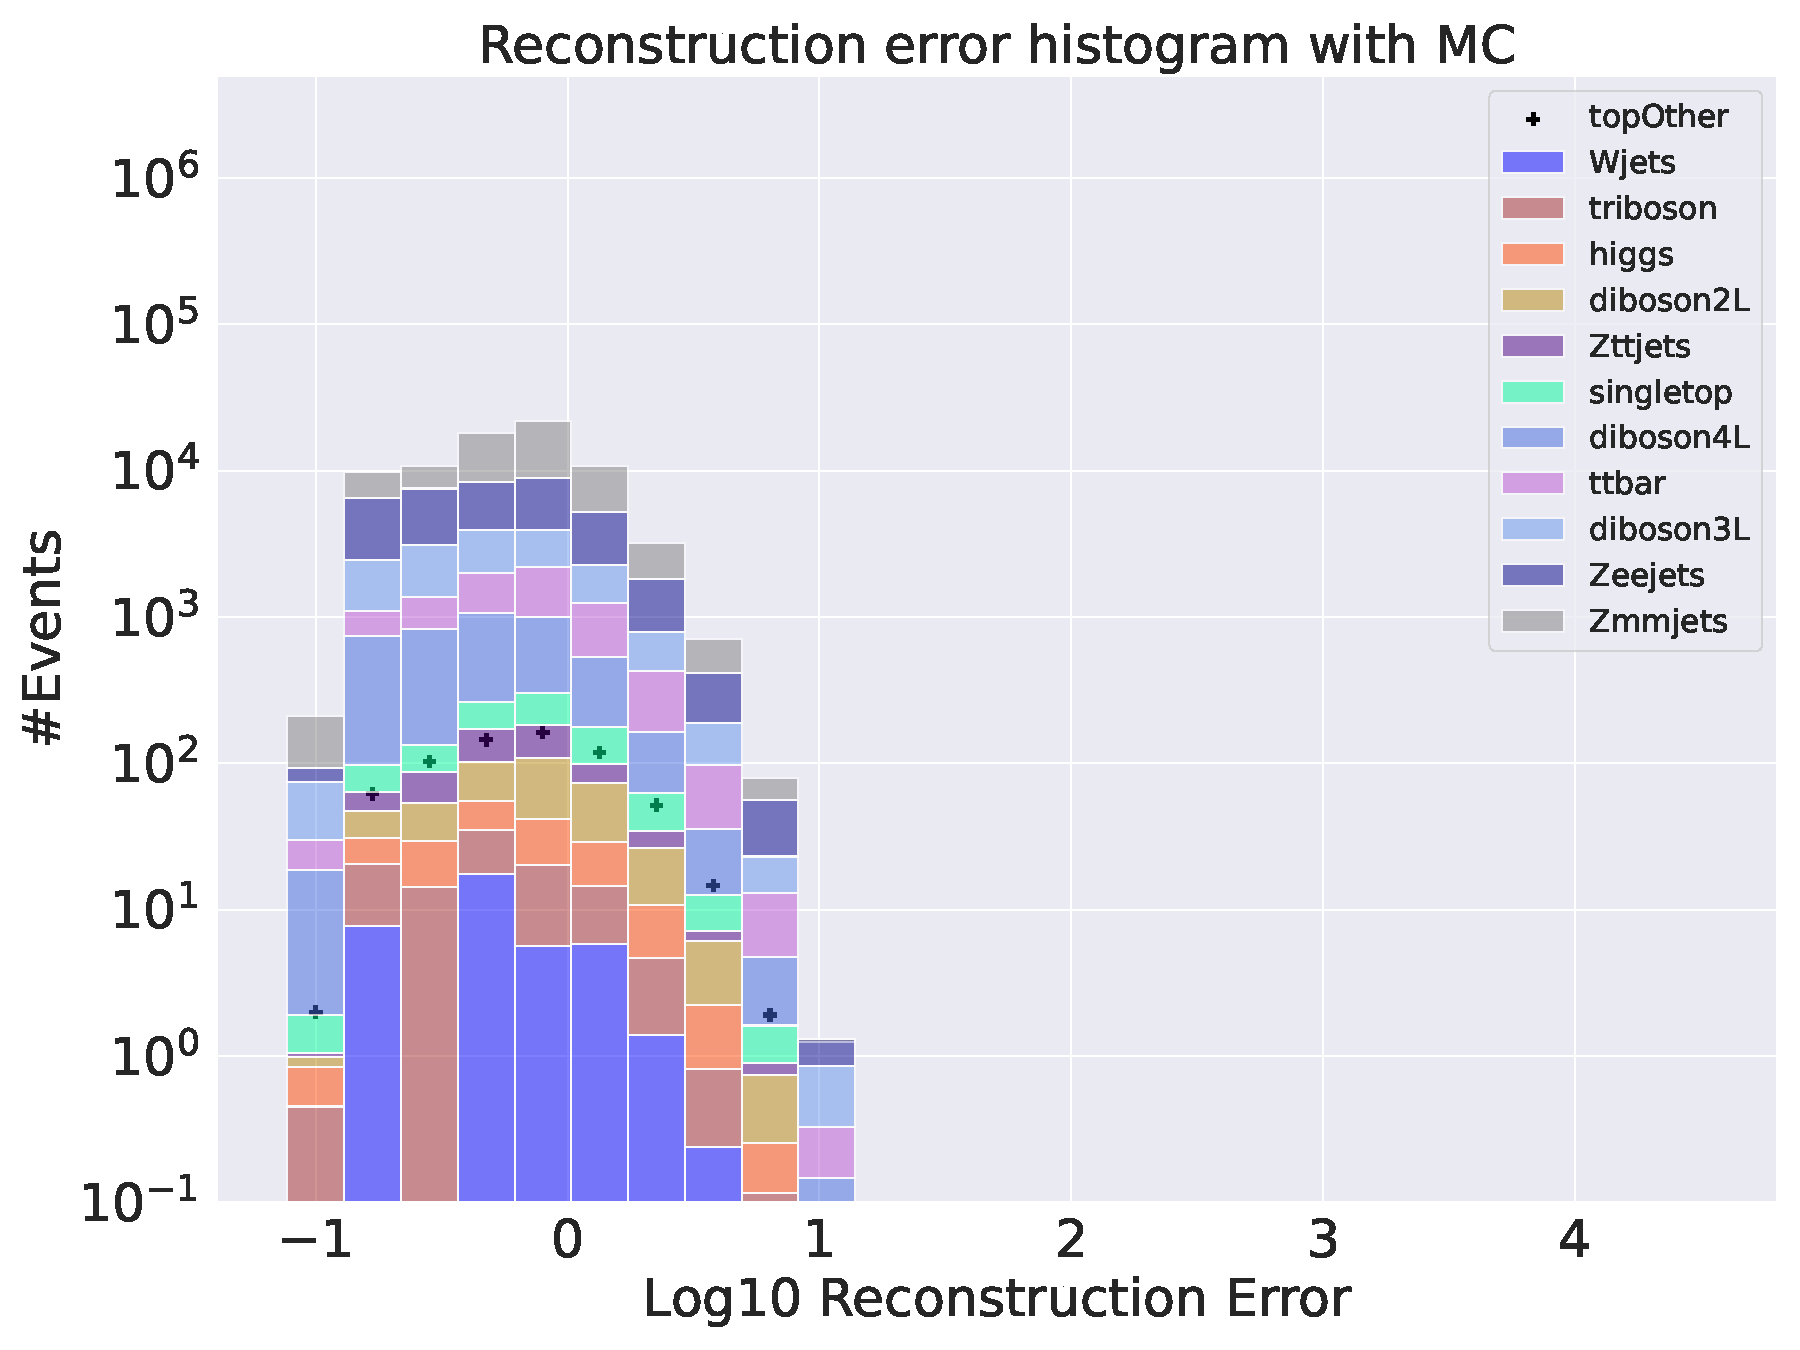
\includegraphics[width=\textwidth]{Figures/VAE_testing/small/b_data_recon_big_rm3_feats_sig_topOther.pdf}
        \caption{Reconstruction error on validation SM MC from the small Autoencoder. Here the topOther channel has been removed from training and 
        is used as signal. No significant difference in distributions are found. }
        \label{fig:vae_small_topOther}
    \end{subfigure}
    \hfill
    \begin{subfigure}{.45\textwidth}
        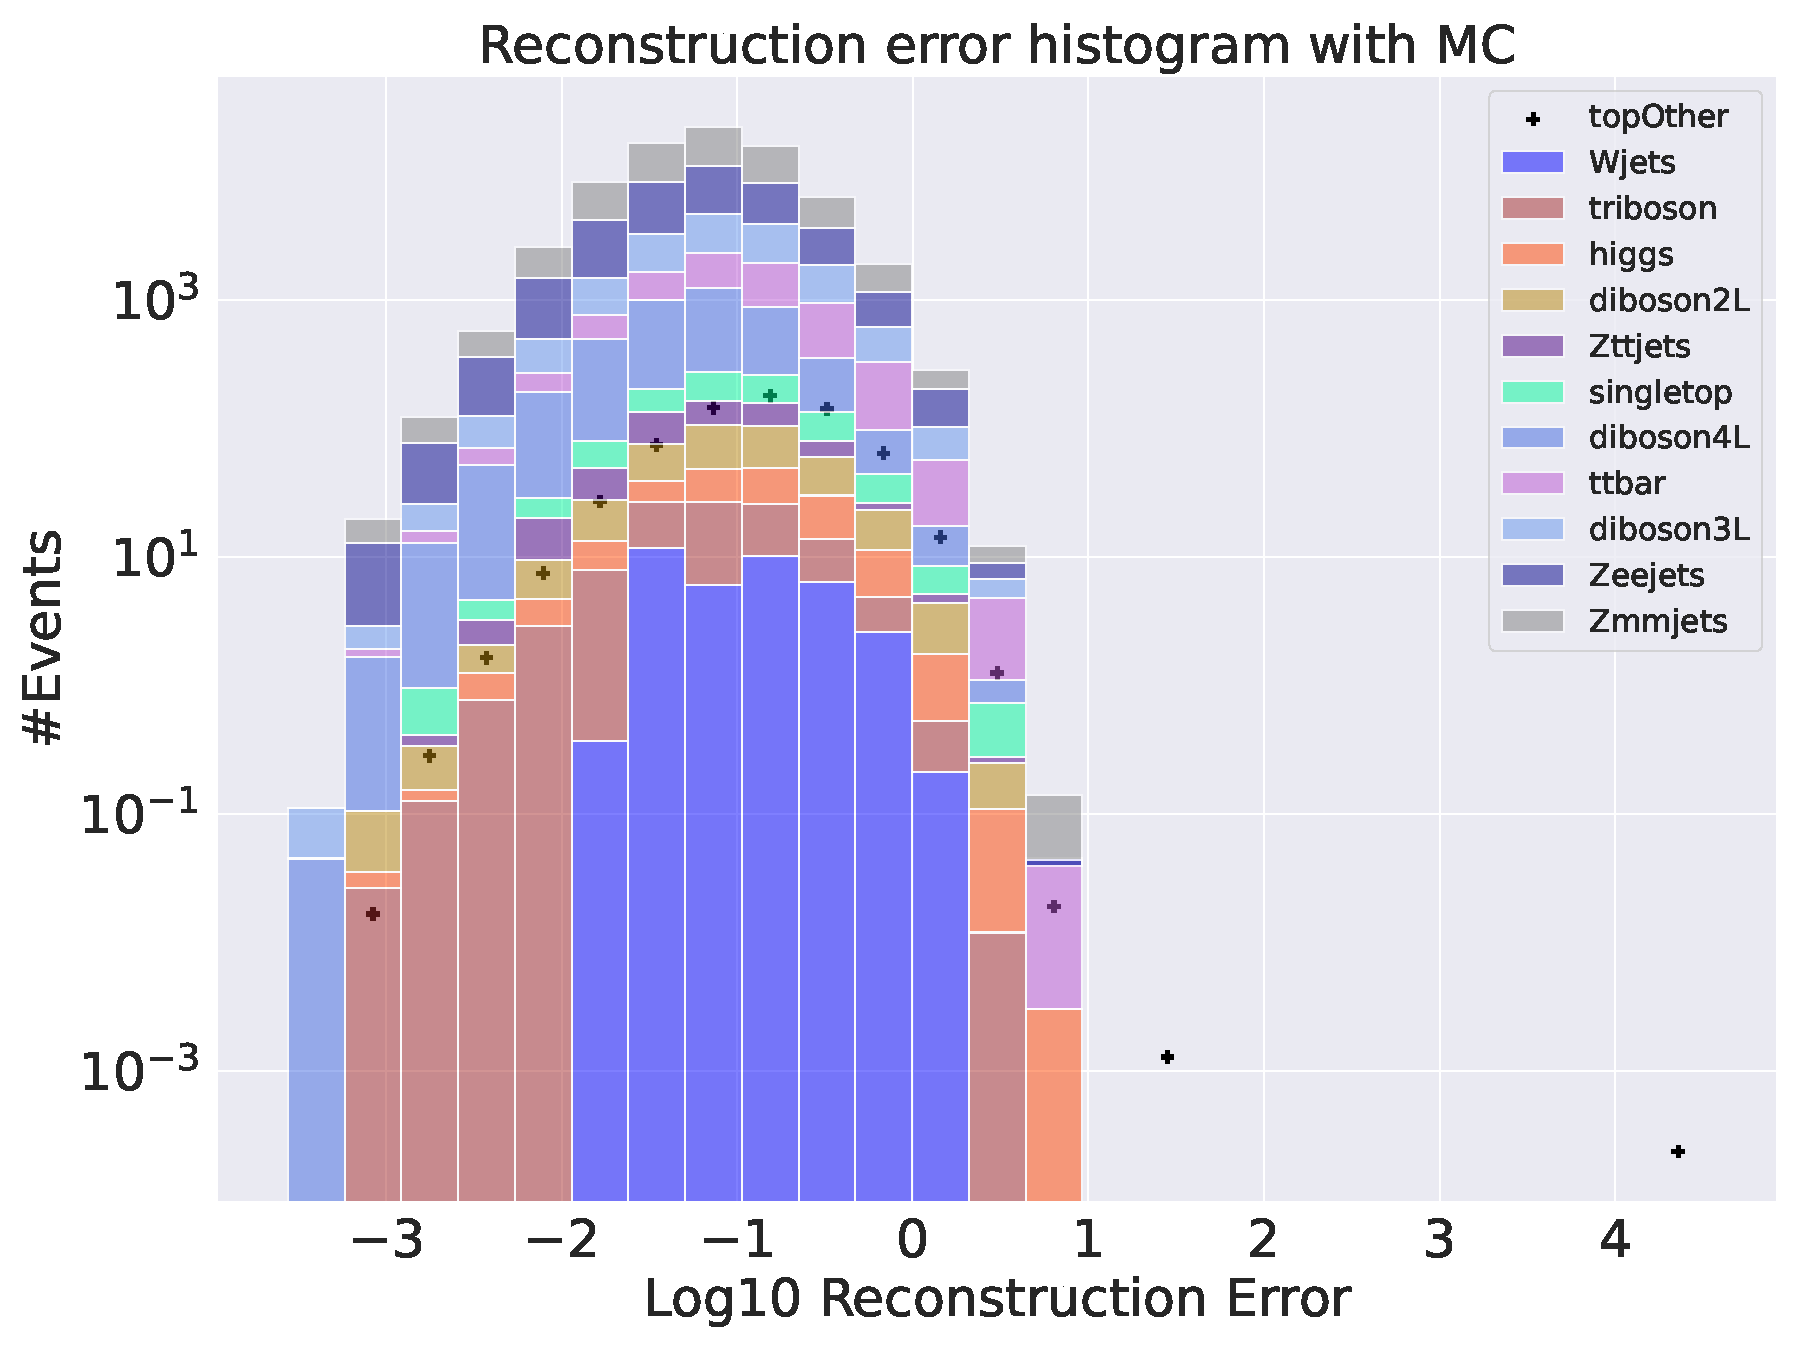
\includegraphics[width=\textwidth]{Figures/VAE_testing/big/b_data_recon_big_rm3_feats_sig_topOther.pdf}
        \caption{Reconstruction error on validation SM MC from the big Autoencoder. Here the topOther channel has been removed from training and 
        is used as signal. No significant difference in distributions are found. }
        \label{fig:vae_big_topOther}
    \end{subfigure}
    \hfill
    \begin{subfigure}{.45\textwidth}
        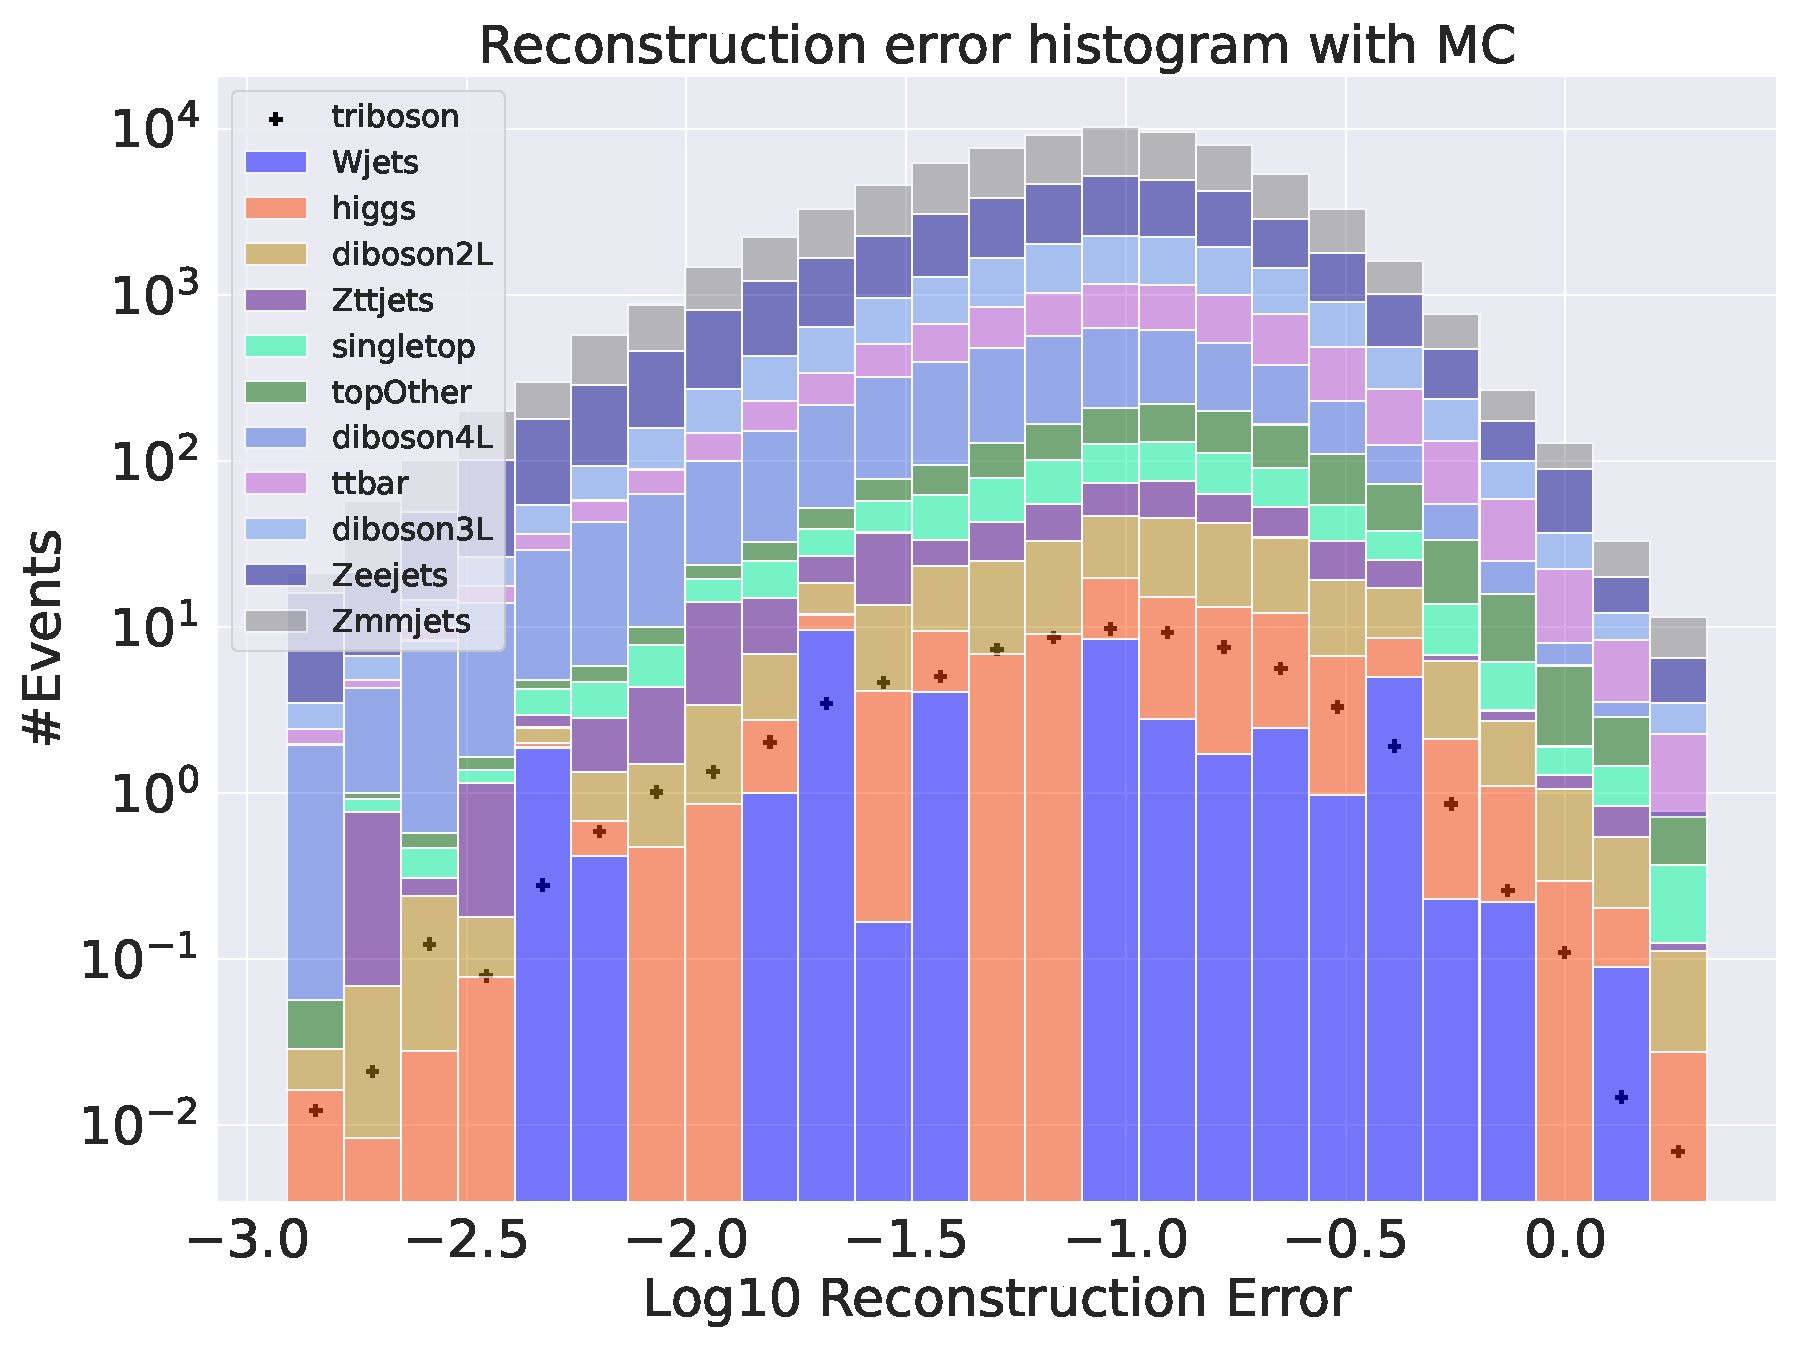
\includegraphics[width=\textwidth]{Figures/VAE_testing/small/b_data_recon_big_rm3_feats_sig_triboson.pdf}
        \caption{Reconstruction error on validation SM MC from the small Autoencoder. Here the triboson channel has been removed from training and 
        is used as signal. No significant difference in distributions are found. }
        \label{fig:vae_small_triboson}
    \end{subfigure}
    \hfill 
    \begin{subfigure}{.45\textwidth}
        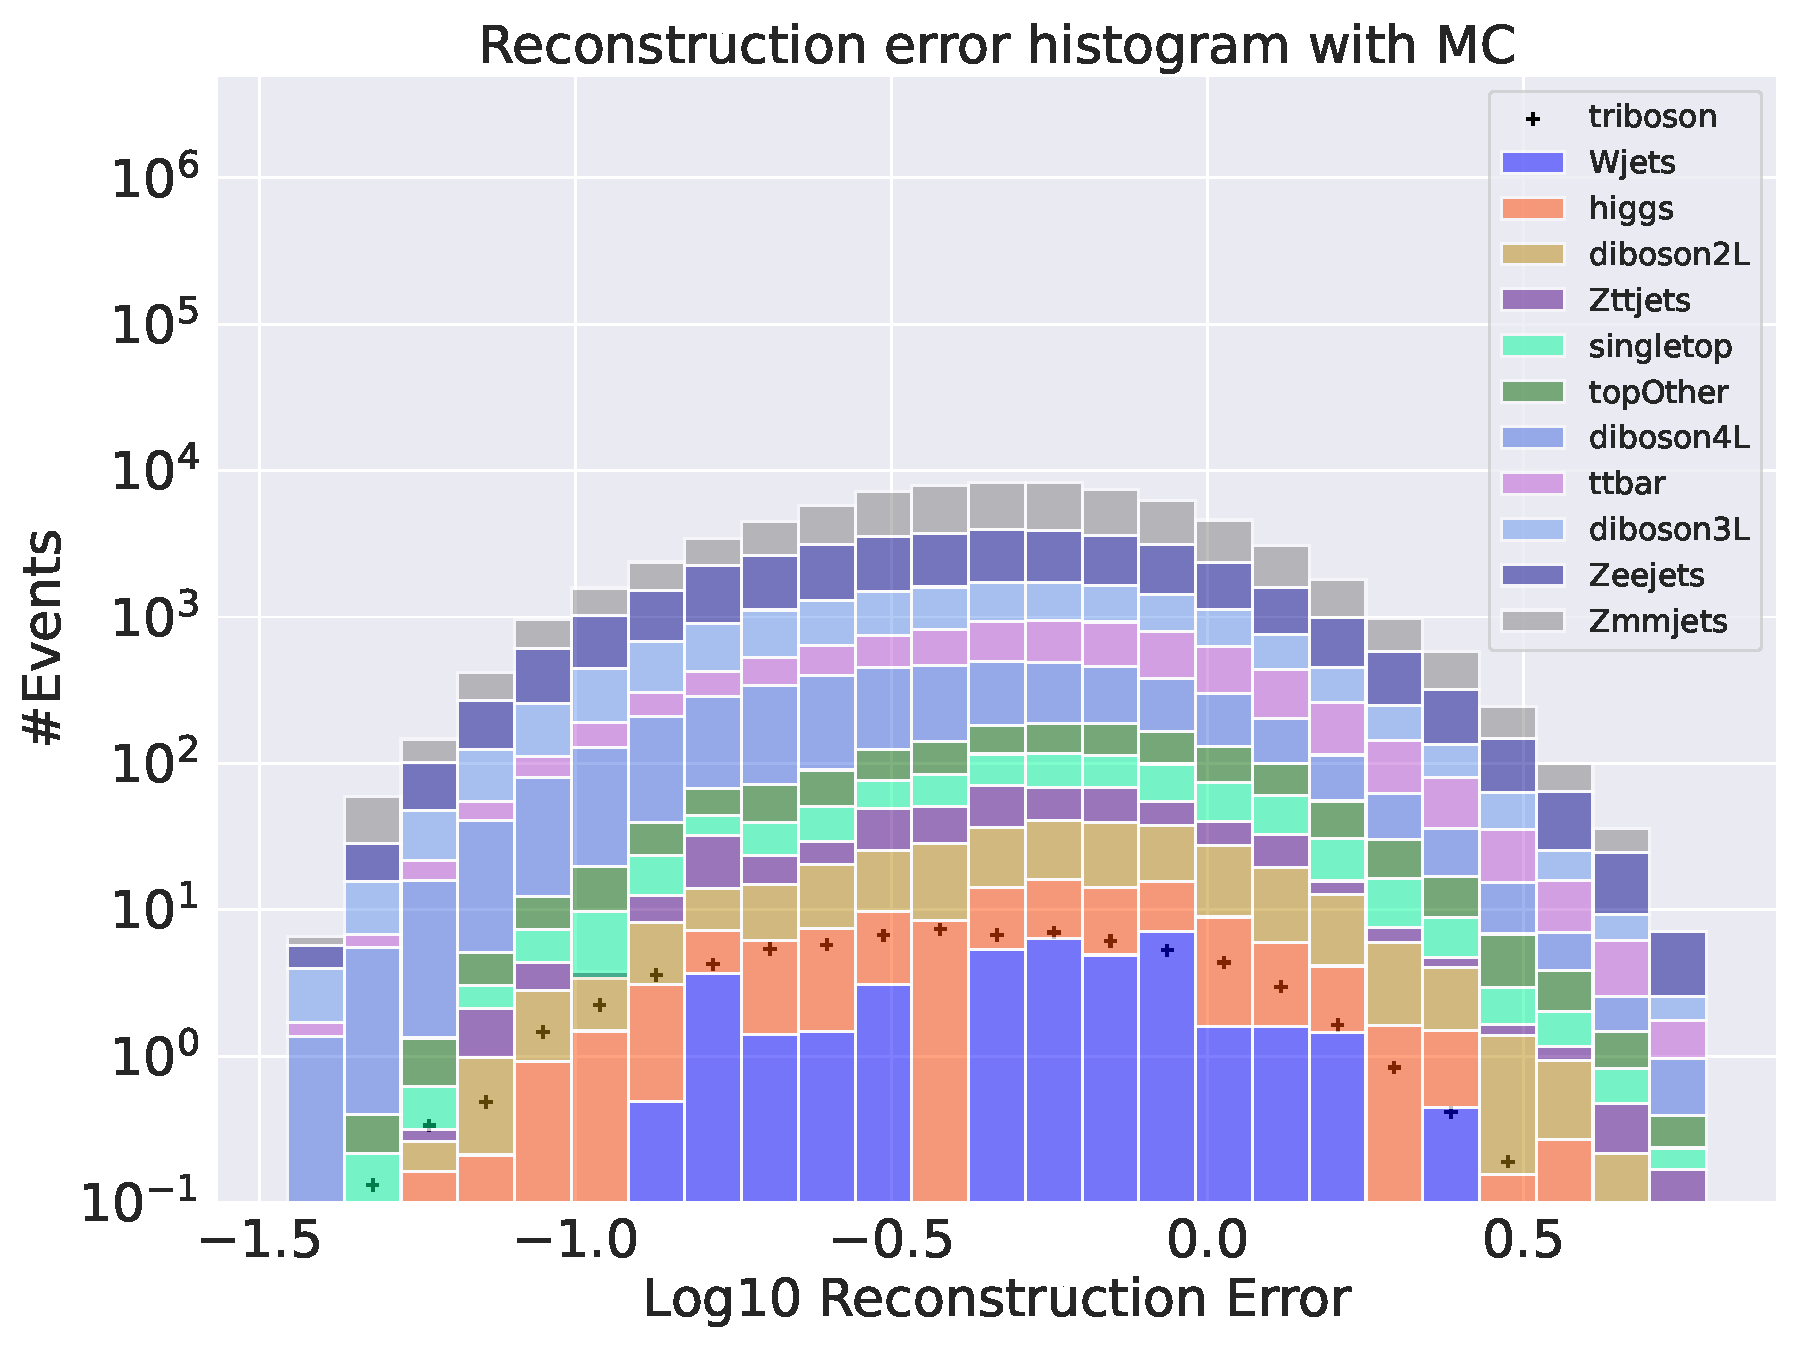
\includegraphics[width=\textwidth]{Figures/VAE_testing/big/b_data_recon_big_rm3_feats_sig_triboson.pdf}
        \caption{Reconstruction error on validation SM MC from the big Autoencoder. Here the triboson channel has been removed from training and 
        is used as signal. No significant difference in distributions are found. }
        \label{fig:vae_big_triboson}
    \end{subfigure}
    \hfill  
    \caption{ }
    \label{fig:vae_big_channel4}
\end{figure}

\begin{figure}[H]
    \centering
    \begin{subfigure}{.45\textwidth}
        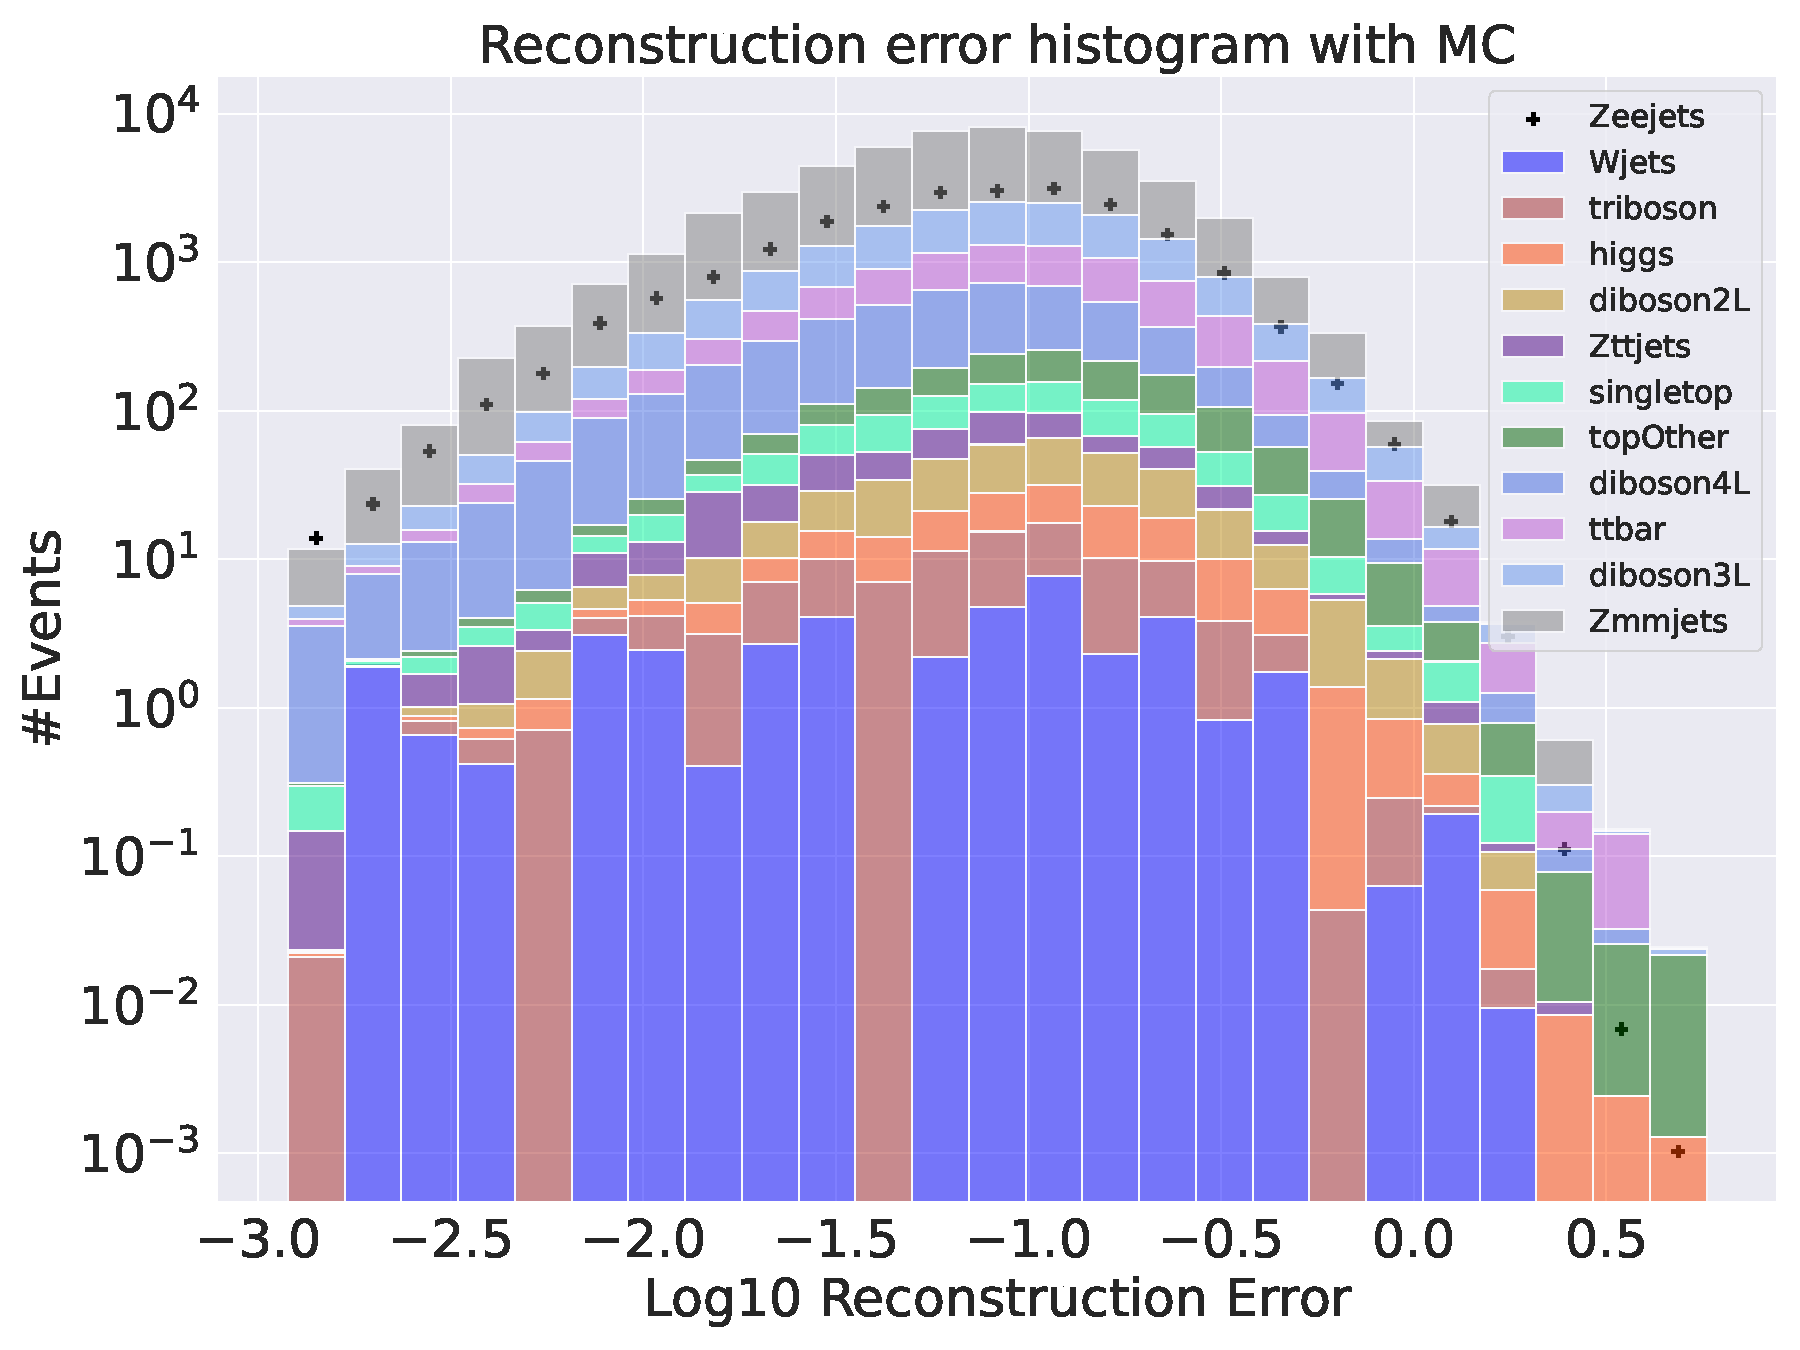
\includegraphics[width=\textwidth]{Figures/VAE_testing/small/b_data_recon_big_rm3_feats_sig_Zeejets.pdf}
        \caption{Reconstruction error on validation SM MC from the small Autoencoder. Here the Zeejets channel has been removed from training and 
        is used as signal. No significant difference in distributions are found.}
        \label{fig:vae_small_Zeejets}
    \end{subfigure}
    \hfill 
    \begin{subfigure}{.45\textwidth}
        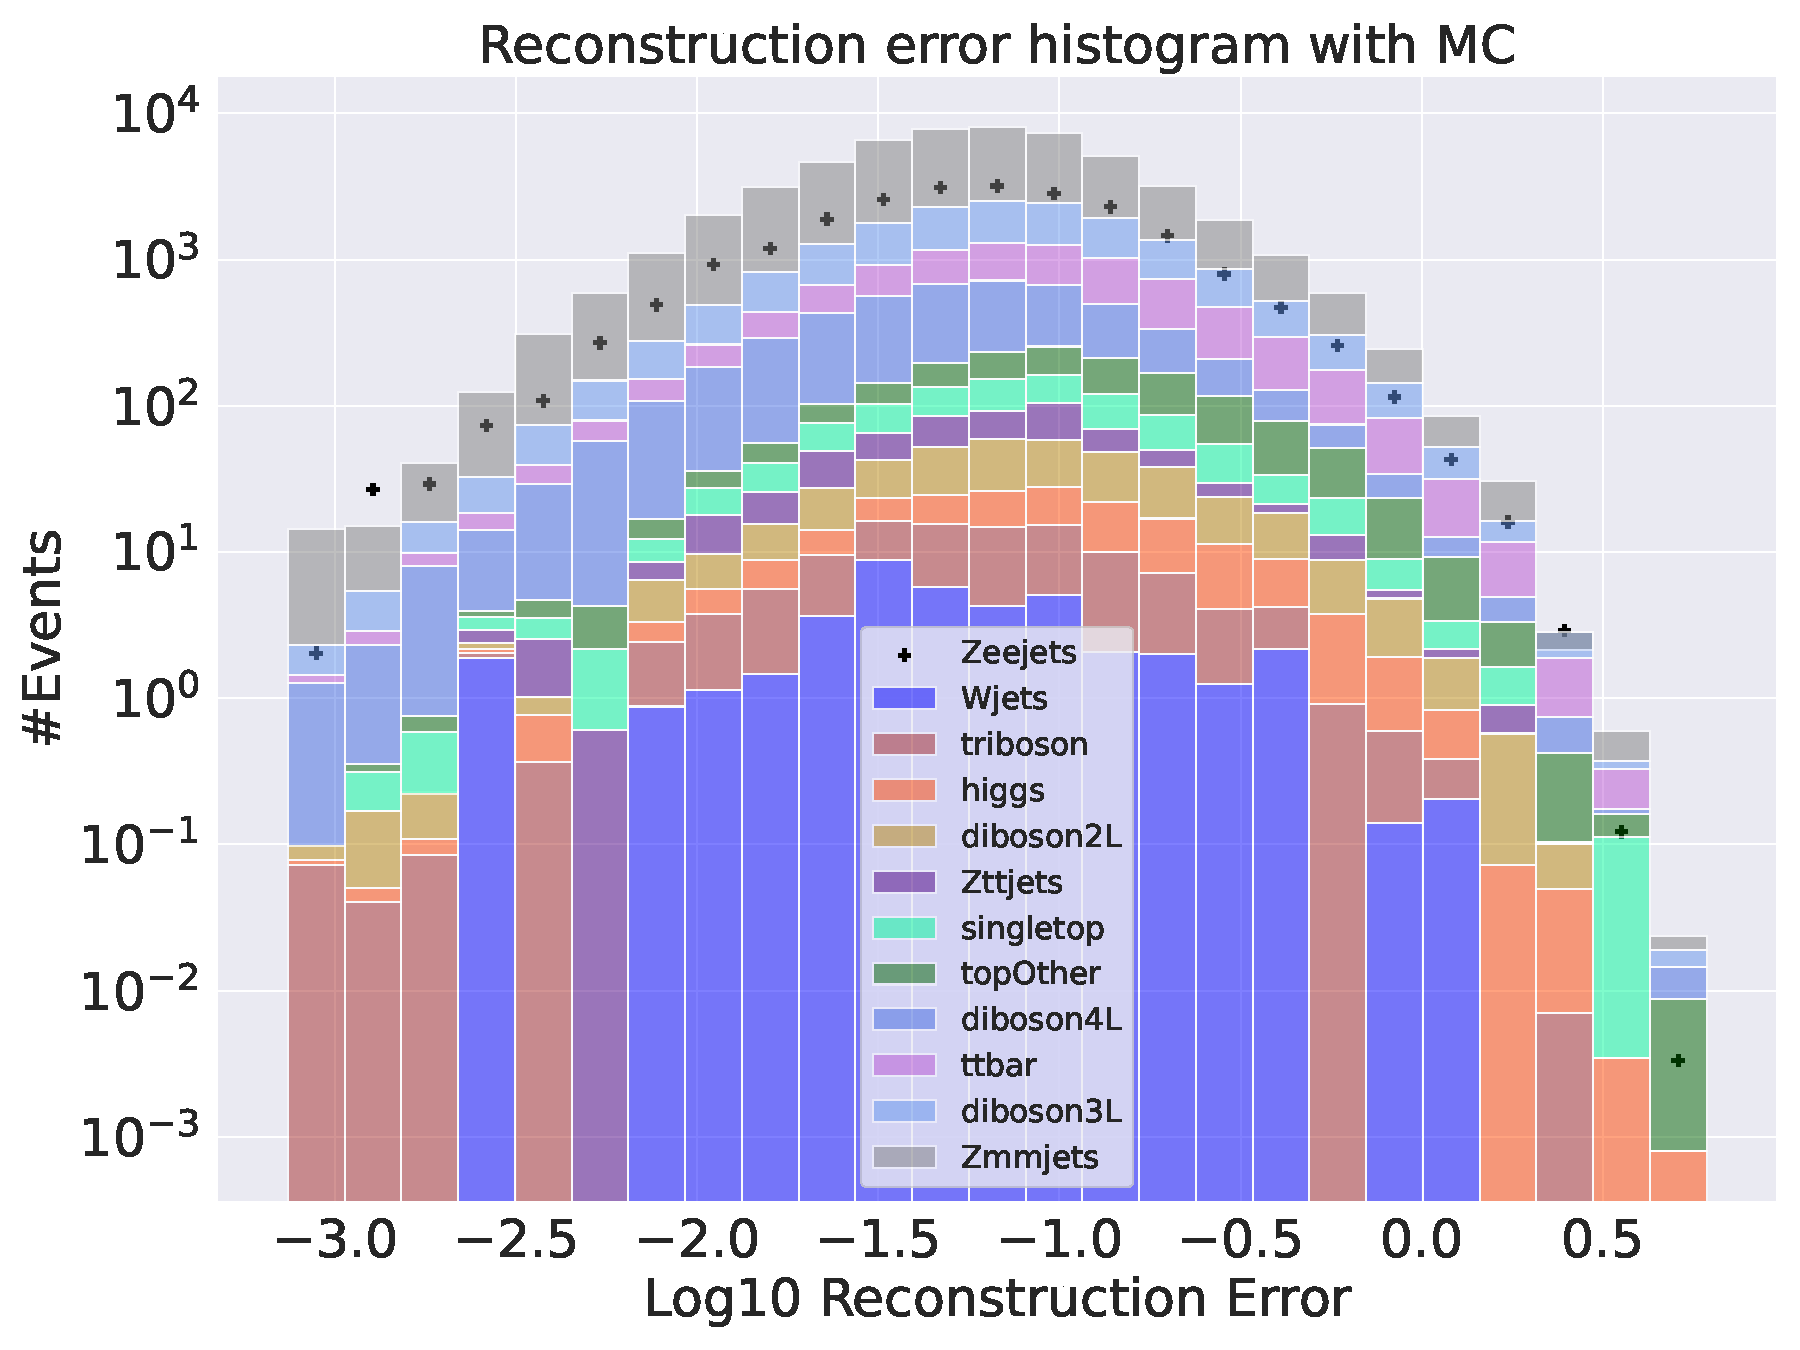
\includegraphics[width=\textwidth]{Figures/VAE_testing/big/b_data_recon_big_rm3_feats_sig_Zeejets.pdf}
        \caption{Reconstruction error on validation SM MC from the big Autoencoder. Here the Zeejets channel has been removed from training and 
        is used as signal. No significant difference in distributions are found. }
        \label{fig:vae_big_Zeejets}
    \end{subfigure}
    \hfill 
    \begin{subfigure}{.45\textwidth}
        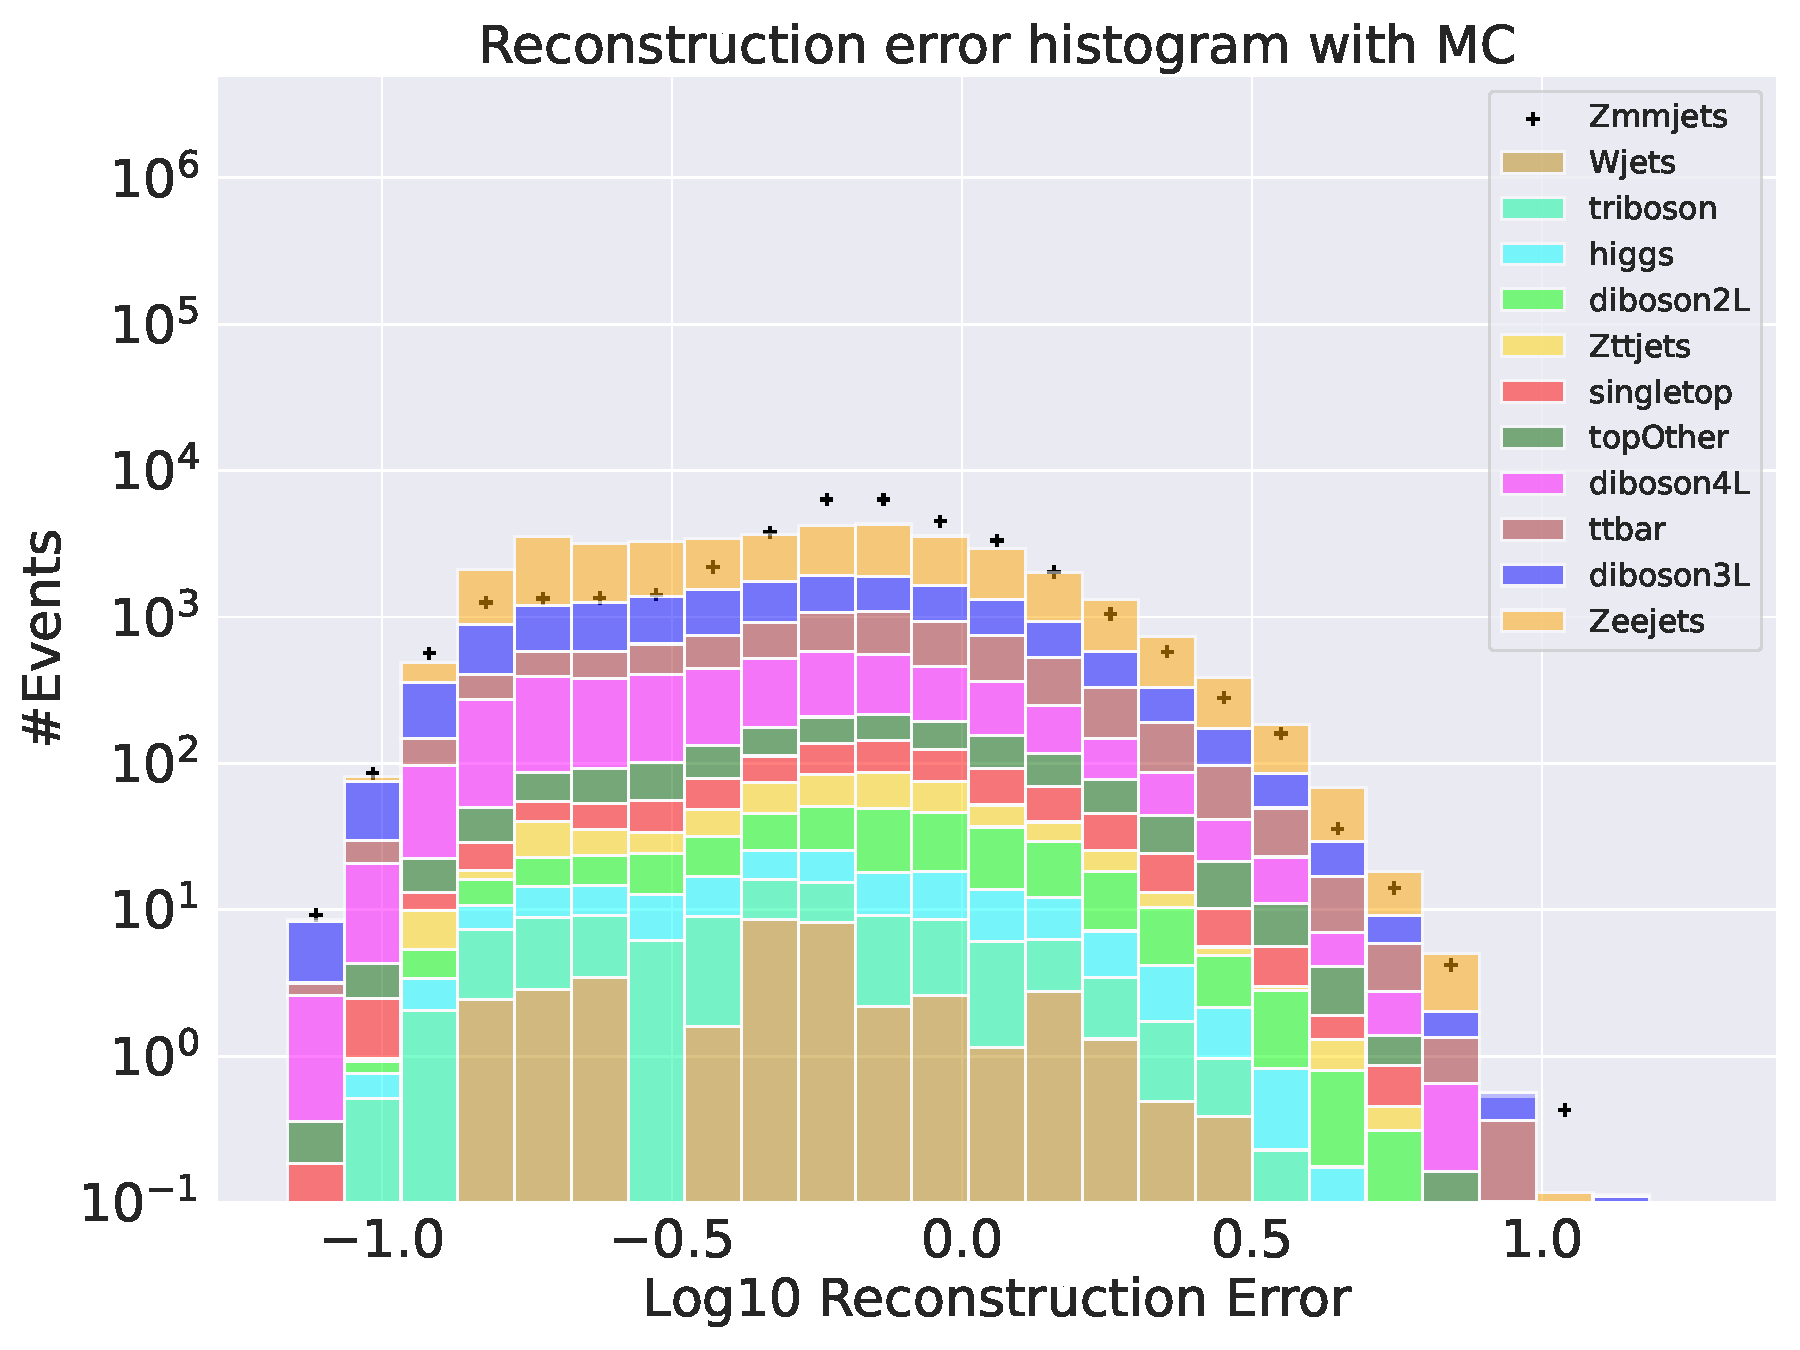
\includegraphics[width=\textwidth]{Figures/VAE_testing/small/b_data_recon_big_rm3_feats_sig_Zmmjets.pdf}
        \caption{Reconstruction error on validation SM MC from the small Autoencoder. Here the Zmmjets channel has been removed from training and 
        is used as signal. No significant difference in distributions are found. }
        \label{fig:vae_small_Zmmjets}
    \end{subfigure}
    \hfill
    \begin{subfigure}{.45\textwidth}
        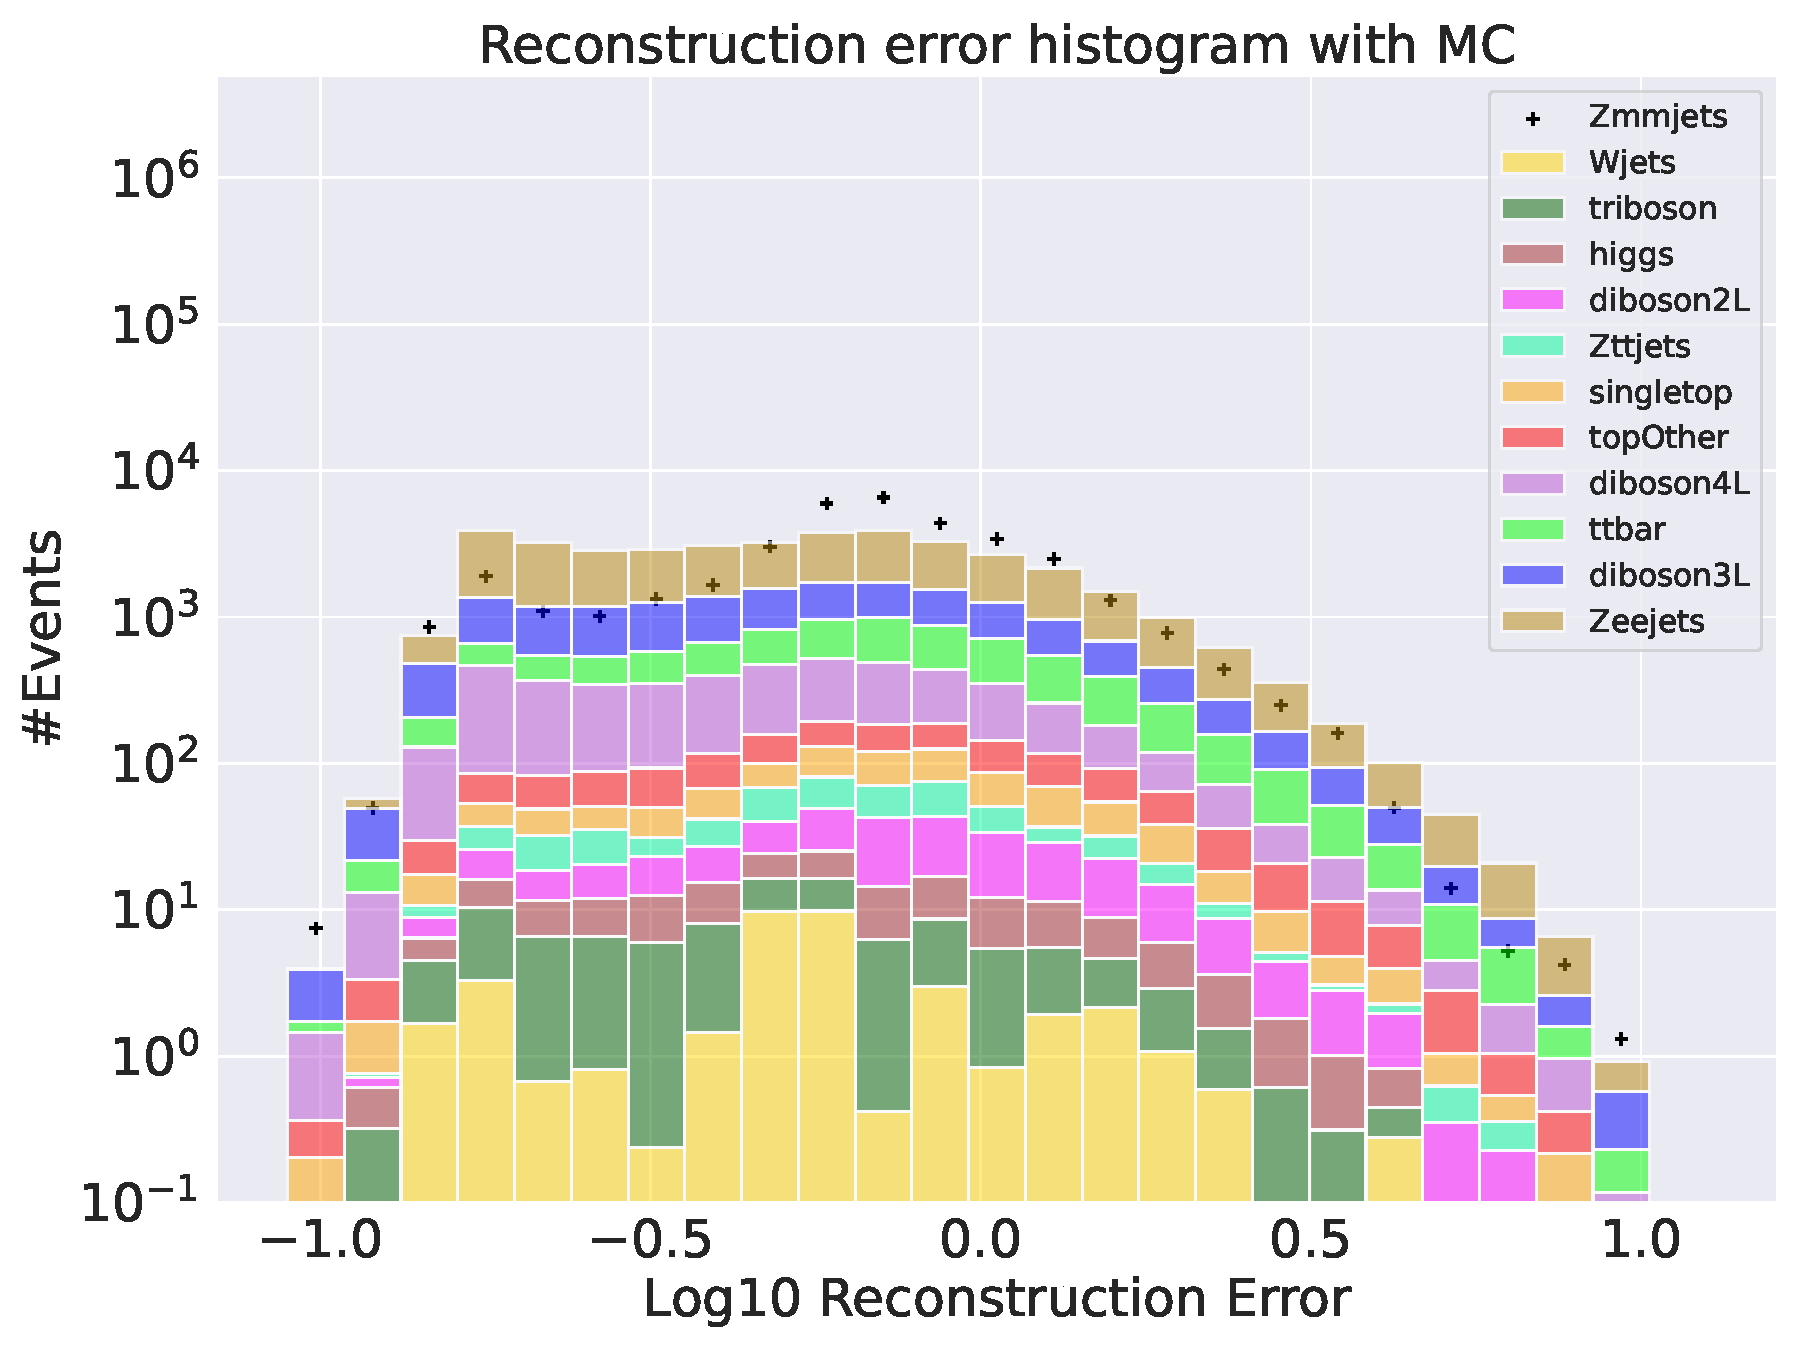
\includegraphics[width=\textwidth]{Figures/VAE_testing/big/b_data_recon_big_rm3_feats_sig_Zmmjets.pdf}
        \caption{Reconstruction error on validation SM MC from the big Autoencoder. Here the Zmmjets channel has been removed from training and 
        is used as signal. No significant difference in distributions are found. }
        \label{fig:vae_big_Zmmjets}
    \end{subfigure}
    \hfill
    \begin{subfigure}{.45\textwidth}
        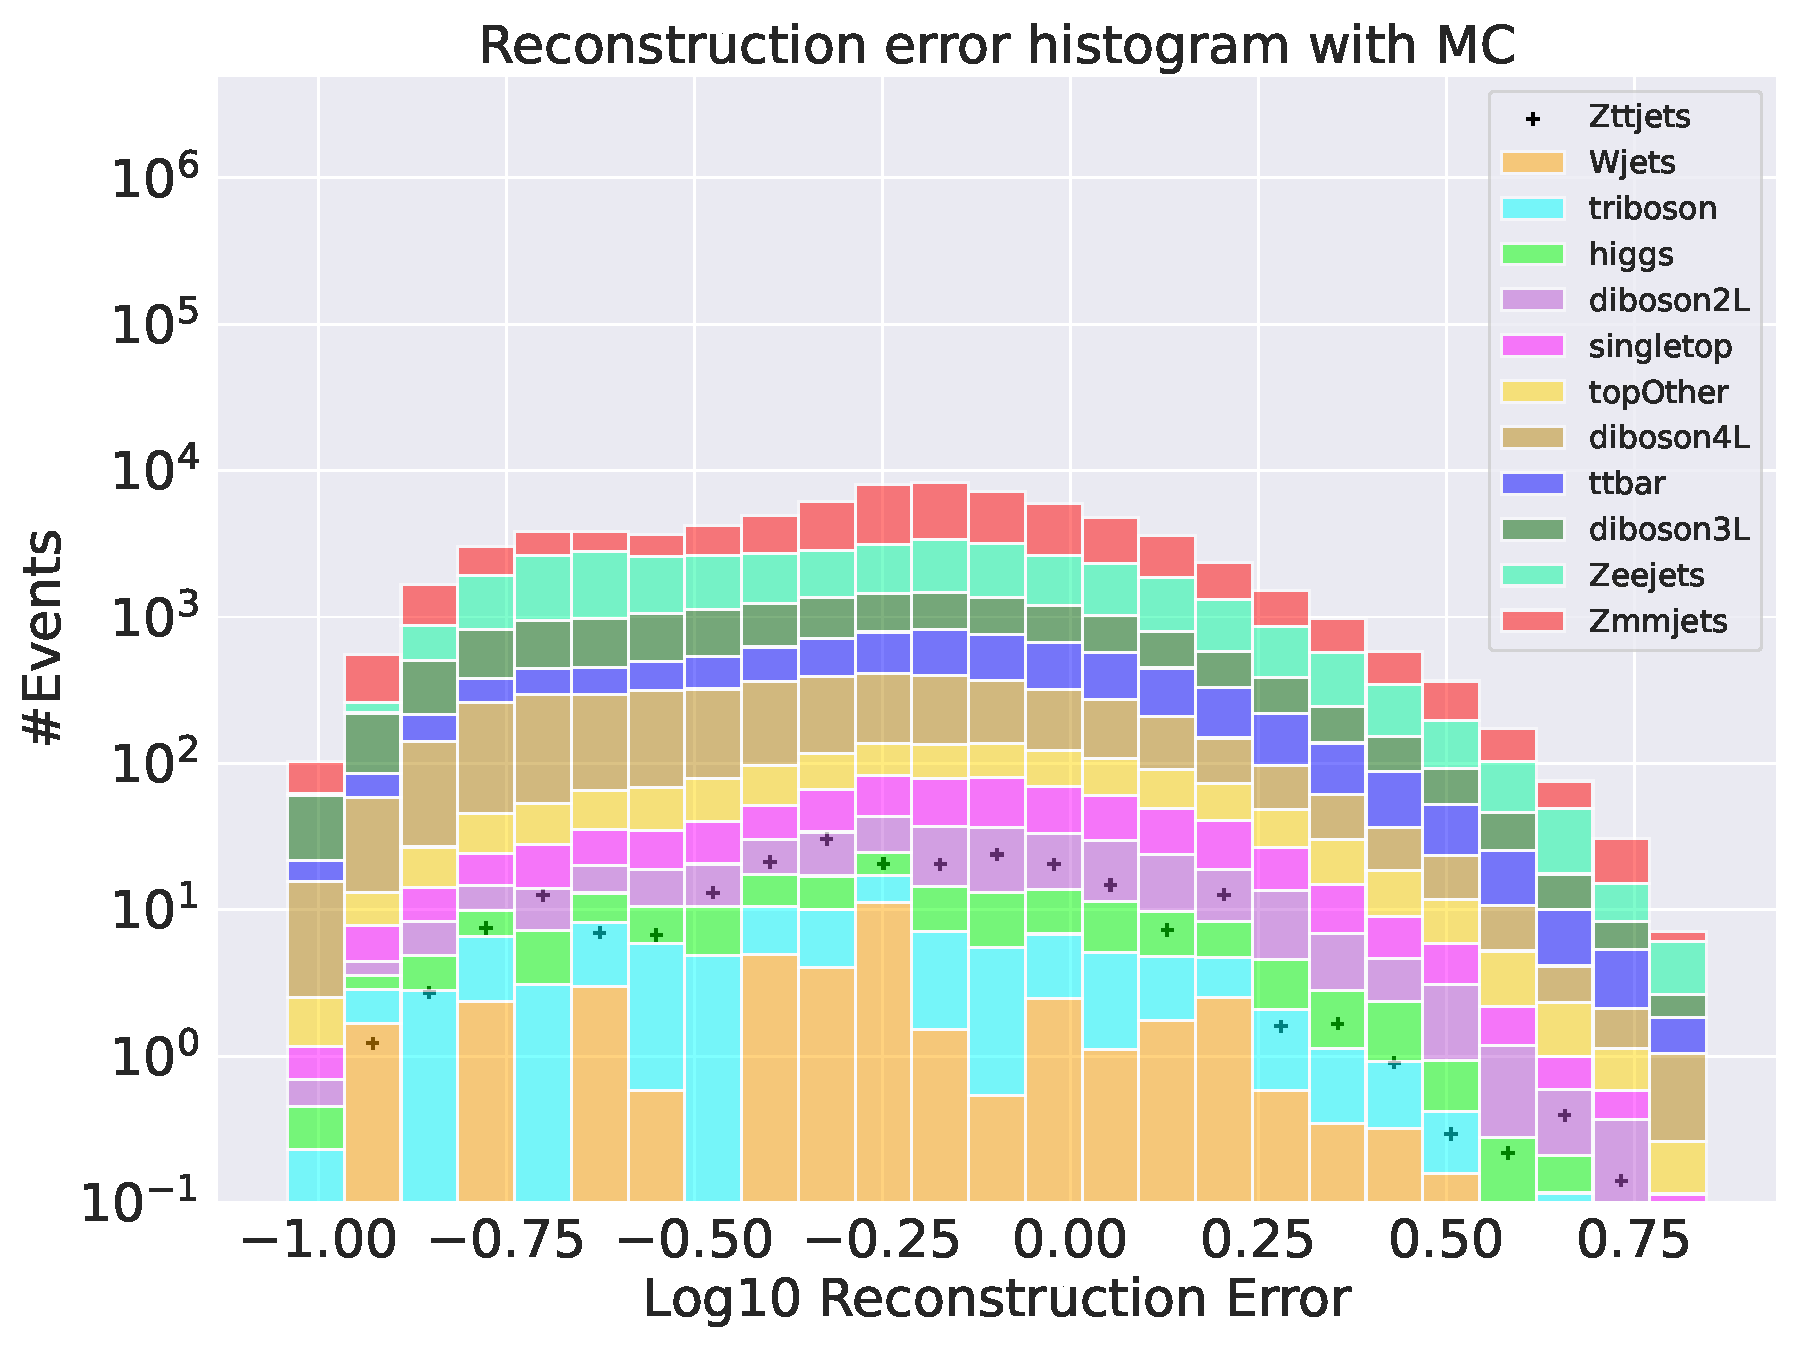
\includegraphics[width=\textwidth]{Figures/VAE_testing/small/b_data_recon_big_rm3_feats_sig_Zttjets.pdf}
        \caption{Reconstruction error on validation SM MC from the small Autoencoder. Here the Zttjets channel has been removed from training and 
        is used as signal. No significant difference in distributions are found. }
        \label{fig:vae_small_Zttjets}
    \end{subfigure}
    \hfill 
    \begin{subfigure}{.45\textwidth}
        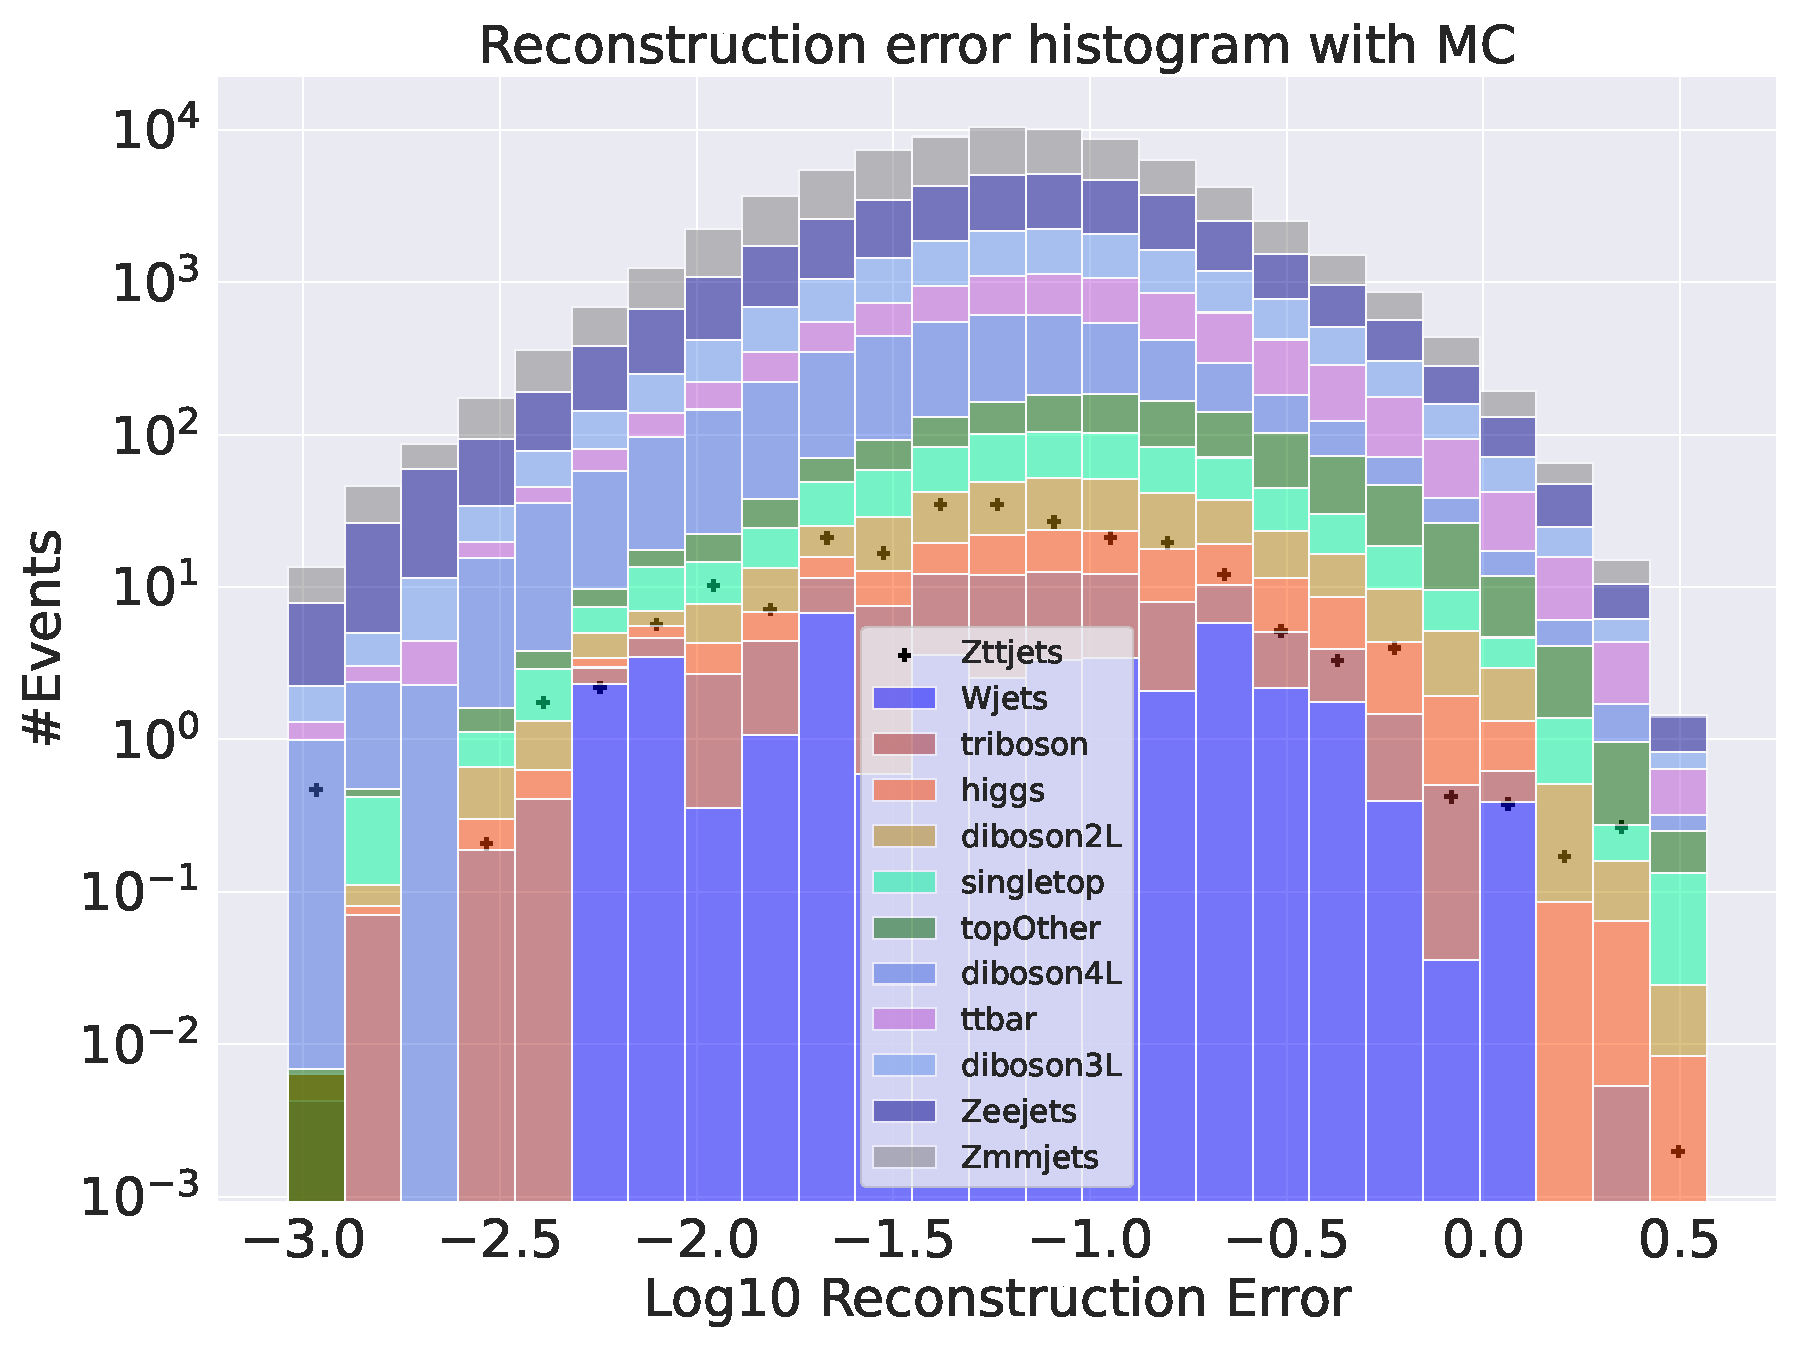
\includegraphics[width=\textwidth]{Figures/VAE_testing/big/b_data_recon_big_rm3_feats_sig_Zttjets.pdf}
        \caption{Reconstruction error on validation SM MC from the big Autoencoder. Here the Zttjets channel has been removed from training and 
        is used as signal. No significant difference in distributions are found. }
        \label{fig:vae_big_Zttjets}
    \end{subfigure}
    \hfill  
    \caption{ }
    \label{fig:vae_big_channel5}
\end{figure}